% =============================================================================
% SOM_dune_development_draft.tex
% Draft manuscript: Effects of Soil Organic Matter on Dune Development
% Following Nature-Based Restoration with Alternative Sediments
% =============================================================================
\documentclass[12pt, a4paper]{article}

% --- Packages ---
\usepackage[utf8]{inputenc}
\usepackage[T1]{fontenc}
\usepackage{amsmath, amssymb}
\usepackage{graphicx}
\graphicspath{{figures/}}
\usepackage[margin=2.5cm]{geometry}
\usepackage{natbib}
\usepackage{booktabs}
\usepackage{siunitx}
\usepackage{lineno}
\usepackage{setspace}
\usepackage{xcolor}
\usepackage{hyperref}
\usepackage{cleveref}
\usepackage{multirow}
\usepackage{longtable}
\usepackage{subcaption}

\hypersetup{
    colorlinks=true,
    linkcolor=blue,
    citecolor=blue,
    urlcolor=blue
}

% APA-style hanging indent for reference list
\newenvironment{hangparas}[2]
  {\setlength{\parindent}{#1}%
   \everypar={\hangindent=\parindent}}
  {}

\doublespacing
\linenumbers

% --- Convenience commands ---
\newcommand{\SOM}{\mathrm{SOM}}
\newcommand{\ust}{u_{*t}}
\newcommand{\usw}{u_{*}}
\newcommand{\todo}[1]{\textcolor{red}{\textbf{[TODO: #1]}}}

% =============================================================================
\begin{document}

% --- Title ---
\title{Optimizing Alternative Sediments for Dune Construction: An Eco-Geomorphological Approach}

\author{
Frederik Van~Daele$^{1,*}$\thanks{Corresponding author: frederik.vandaele@ugent.be} \and
Charlotte Taelman$^{2}$ \and
Maaike Dhondt$^{2}$ \and
Jianghua Guo$^{3}$ \and
Jiayue Yan$^{2}$ \and
Katrien Vanderbiest$^{4}$ \and
Pieter Rauwoens$^{3}$ \and
Dries Bonte$^{2}$
}

\date{
$^{1}$Department of Civil Engineering, Ghent University, Belgium \\
$^{2}$Department of Biology, Ghent University, Belgium \\
$^{3}$Department of Civil Engineering, KU Leuven, Technology Campus Bruges, Belgium \\
$^{4}$University of Antwerp, Belgium \\[0.5em]
\today~--- \textbf{Draft manuscript for internal review}
}

\maketitle

% =============================================================================
% ABSTRACT
% =============================================================================
\begin{abstract}
Nature-based solutions for coastal protection increasingly rely on dune-in-front-of-dike (DfD) systems constructed with sand from dredging operations. However, the long-term geomorphological development of dunes built with organic-rich alternative sediments remains poorly understood. We present an integrated experimental--numerical framework that couples (i) common-garden and germination experiments quantifying marram grass (\textit{Calamagrostis arenaria}) performance on 10 substrate mixtures varying in soil organic matter (SOM) content (\SIrange{0.06}{2.5}{\percent} total organic carbon), (ii) a process-based aeolian--vegetation feedback model (Living Dunes) extended with dynamic SOM--ecohydrology and SOM--cohesion pathways, and (iii) storm erosion assessment using XBeach. Growth experiments demonstrated that marram grass germination and establishment were significantly enhanced on organic-rich alternative substrates compared to natural beach sand, with leaf counts on the dark dredging substrate exceeding the reference by a factor $>$2. We parameterised the Living Dunes model to simulate three-year dune development at Ostend (Belgium) under 10 sediment scenarios ranging from pure beach sand to pure dredging material. Model extensions included a Saxton and Rawls pedotransfer function linking SOM to field capacity (the ``sponge effect''), a dynamic organic cohesion modifier following Zobeck et al., and a disturbance-recovery index after Belnap and Gillette. Furthermore, we parameterised trait-specific growth functions based on SOM to reflect observed variations in vegetation vigour. Three-year simulations were followed by XBeach storm impact modelling and subsequent Living Dunes recovery simulations to assess the self-restoring capacity of the constructed dunes. Preliminary model results indicate that moderate SOM enrichment (\SIrange{1}{2}{\percent} TOC) optimises both vegetation vigour and aeolian sediment supply, producing the tallest and most erosion-resistant dune profiles, while further increases in organic content progressively suppress aeolian transport through enhanced moisture retention and organic cohesion. These findings provide evidence-based guidelines for the sustainable use of dredging by-products in nature-based coastal defences.

\bigskip
\noindent\textbf{Keywords:} soil organic matter; nature-based solutions; dune restoration; marram grass; alternative sediments; aeolian transport; coastal resilience; Living Dunes model; XBeach
\end{abstract}

\newpage

% =============================================================================
% 1. INTRODUCTION
% =============================================================================
\section{Introduction}

Sandy coastlines provide critical ecosystem services including flood defence, habitat provision, and recreational value \citep{martinez2008coastal}. In low-lying countries such as Belgium, dune-in-front-of-dike (DfD) systems have been proposed as nature-based solutions that combine coastal safety with ecological restoration \citep{temmerman2013ecosystem}. Unlike traditional hard engineering structures, these systems rely on biophysical feedbacks between vegetation, sediment, and wind to build and maintain their protective volume over time \citep{bonte2021biomorphogenic}.

A fundamental requirement for DfD construction is the availability of suitable sediment in sufficient quantities. Sand is, however, a finite and increasingly contested resource. In the Belgian part of the North Sea (BPNS), extraction volumes surged from \SI{0.3e6}{\cubic\metre} in 1976 to \SI{3.5e6}{\cubic\metre} in 2019, and mid-term projections indicate growing scarcity of high-quality aggregates. Only \SI{16}{\percent} of sand used for coastal safety in Flanders originates from beneficial reuse of dredging material, with the remainder sourced from dedicated extraction zones defined in the Marine Spatial Plan \citep{speybroeck2006beach}. This situation has motivated research into whether alternative sediments---particularly by-products from maintenance dredging in ports and navigation channels---can be repurposed for dune construction.

Alternative sediments from dredging typically differ from native beach sand in three principal ways: they have a finer grain size distribution, a higher soil organic matter (SOM) content, and a more heterogeneous texture \citep{vandeneede2014assessing}. Each of these properties influences the aeolian and ecological processes that govern dune development. Finer grains reduce the threshold shear velocity for transport initiation but also increase interparticle cohesion \citep{shao2000simple}. Elevated SOM content enhances soil water retention through increased microporosity \citep{saxton2006soil}, strengthens interparticle bonding via organic polymers and biocrust formation \citep{zobeck2013soil}, and alters nutrient availability for vegetation establishment \citep{vanderputten1993plant}. Understanding these interacting effects is essential for predicting whether DfD systems constructed with alternative sediments will develop into functional, self-sustaining dunes.

Marram grass (\textit{Calamagrostis arenaria}, formerly \textit{Ammophila arenaria}) is the dominant ecosystem engineer in northwest European foredunes. It traps wind-blown sand through aerodynamic roughness and drag, and responds positively to moderate sand burial through stimulated vertical and lateral growth \citep{huiskes1979ammophila, disraeli1984effect, keijsers2016adaptation, reijers2021review}. This positive feedback between vegetation growth and sand accretion makes marram grass the keystone species for dune building. However, how marram grass responds to substrates with elevated organic matter---specifically whether the improved moisture retention and nutrient supply compensate for potentially reduced aeolian sand supply---remains an open question.

Previous studies on beach nourishment ecology have focused primarily on intertidal macrofauna response to sediment grain size \citep{speybroeck2006beach, vandeneede2014assessing}. Research on dune vegetation establishment on alternative substrates has been limited to qualitative field observations, and no study has quantitatively linked substrate organic matter content to dune geomorphological development through both experimental and numerical approaches.

The SUSANA project (Sustainable Use of Sand in Nature-based Solutions) addresses this gap through a multi-partner research programme that combines field experiments, laboratory analyses, and numerical modelling. The present study integrates three complementary research lines. First, we report the results of common-garden and germination experiments testing marram grass performance on 10 substrate mixtures spanning the range from pure natural beach sand to pure dredging material, conducted at the port of Zeebrugge over one growing season. Second, we describe extensions to the Living Dunes model---a spatially explicit, process-based aeolian--vegetation feedback model---that represent the effects of SOM on soil moisture retention, threshold shear velocity, and surface disturbance dynamics. Third, we apply this model to simulate three-year dune development at a DfD site near Ostend under each of the 10 substrate scenarios, followed by XBeach storm erosion modelling and post-storm recovery simulations to assess the self-restoring capacity of the resulting dune profiles.

The primary objectives of this study are to (1) quantify the effect of substrate SOM content on marram grass establishment and growth, (2) develop and validate a modelling framework that captures the coupled effects of SOM on ecohydrology and aeolian transport, and (3) identify the SOM range that optimises long-term dune development and storm resilience. We hypothesise that SOM acts as a ``double-edged sword'' for dune development, where enhanced moisture retention promotes vegetation growth but simultaneously suppresses the aeolian sediment supply necessary for continued dune building. Together, these results provide evidence-based recommendations for the use of alternative sediments in nature-based coastal defence.


% =============================================================================
% 2. METHODS
% =============================================================================
\section{Methods}

\subsection{Study Area}

The study site is located along the central Belgian coast near Ostend (51\textdegree12\textquotesingle N, 2\textdegree55\textquotesingle E), where a DfD system was constructed seaward of the existing sea dike. The Belgian coast is a macrotidal, wave-dominated sandy shore oriented northeast--southwest, with a tidal range of approximately \SI{4.5}{\metre} (spring tide) and a prevailing wind direction from the southwest \citep{degraer2006belgian}. The existing beach at Ostend consists of medium-grained quartz sand with a median grain size ($D_{50}$) of approximately \SI{335}{\micro\metre}, a 90th-percentile grain diameter ($D_{90}$) of \SI{500}{\micro\metre}, and a bulk density of \SI{1500}{\kilo\gram\per\cubic\metre}. Common-garden experiments were conducted at the port of Zeebrugge (51\textdegree20\textquotesingle N, 3\textdegree10\textquotesingle E), approximately \SI{25}{\kilo\metre} northeast of Ostend, which shares the same coastal climate regime.


\subsection{Substrate Characterisation}

Ten substrates were analysed for use in both the experimental and modelling components of this study. These comprised natural beach sand from Zeebrugge (designated R, the reference substrate), a dark-coloured alternative substrate from port dredging (D), a white-coloured alternative substrate (W), and seven mixtures of D and W (\cref{tab:substrate_properties}). Five samples were analysed per substrate type for total organic carbon (TOC), total nitrogen (TN), and median grain size ($D_{50}$); samples were dried at \SI{60}{\degreeCelsius} for 24 hours prior to analysis, and granulometry was restricted to the fraction $<$\SI{2}{\milli\metre}.

The alternative substrates exhibited markedly different properties from the reference beach sand (\cref{tab:substrate_properties}). The dark substrate (D) had the highest TOC content (\SI{2.16}{\percent}), approximately 36 times greater than the reference sand (\SI{0.06}{\percent}), and the smallest median grain size (\SI{182.9}{\micro\metre}). The white substrate (W) had an intermediate TOC (\SI{0.25}{\percent}) and a grain size (\SI{187.9}{\micro\metre}) closer to but still finer than the reference sand (\SI{266.9}{\micro\metre}). The D/W mixtures spanned a continuous gradient in SOM, grain size, and nitrogen content between these end-members.

\begin{table}[htbp]
\centering
\caption{Physical and chemical properties of the 10 experimental substrates. TOC: total organic carbon; TN: total nitrogen; $D_{50}$: median grain diameter.}
\label{tab:substrate_properties}
\begin{tabular}{lccc}
\toprule
Substrate & TOC (\%) & TN (\%) & $D_{50}$ (\si{\micro\metre}) \\
\midrule
R (reference beach sand) & 0.06 & 0.04 & 266.9 \\
W (white dredge) & 0.25 & 0.07 & 187.9 \\
D12.5 (12.5\% D / 87.5\% W) & 0.49 & 0.09 & 187.3 \\
D25 (25\% D / 75\% W) & 0.73 & 0.10 & 186.6 \\
D37.5 (37.5\% D / 62.5\% W) & 0.97 & 0.12 & 186.0 \\
D50 (50\% D / 50\% W) & 1.21 & 0.13 & 185.4 \\
D62.5 (62.5\% D / 37.5\% W) & 1.45 & 0.14 & 184.8 \\
D75 (75\% D / 25\% W) & 1.68 & 0.16 & 184.2 \\
D87.5 (87.5\% D / 12.5\% W) & 1.92 & 0.17 & 183.5 \\
D (dark dredge) & 2.16 & 0.19 & 182.9 \\
\bottomrule
\end{tabular}
\end{table}

\begin{figure}[htbp]
    \centering
    \begin{subfigure}[b]{0.85\textwidth}
        \centering
        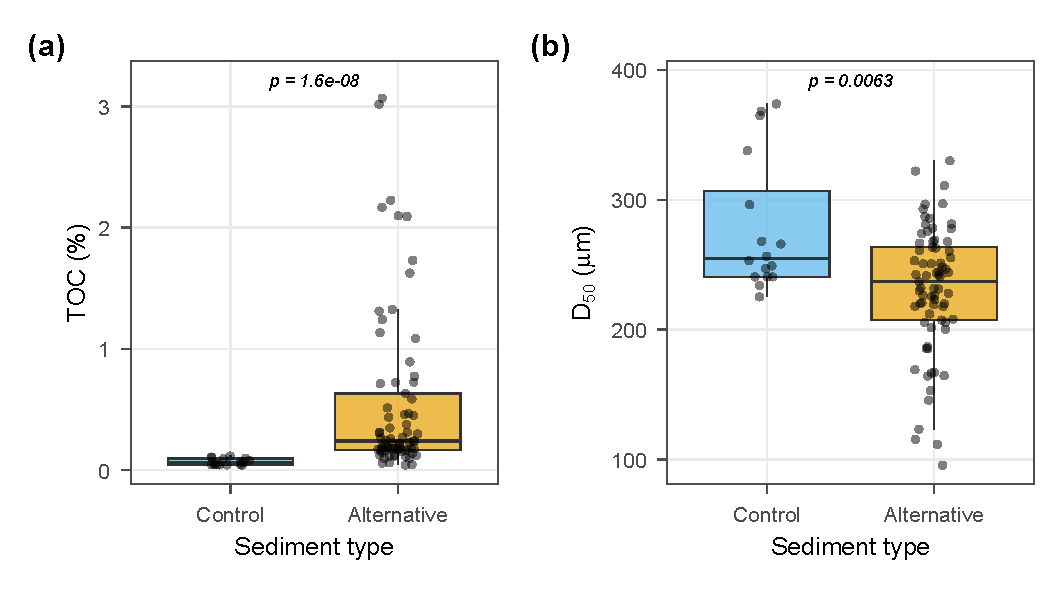
\includegraphics[width=\textwidth]{substrate_toc_d50.pdf}
        \caption{Substrate TOC gradient}
        \label{fig:toc_gradient}
    \end{subfigure}
    \par\vspace{1em}
    \begin{subfigure}[b]{0.85\textwidth}
        \centering
        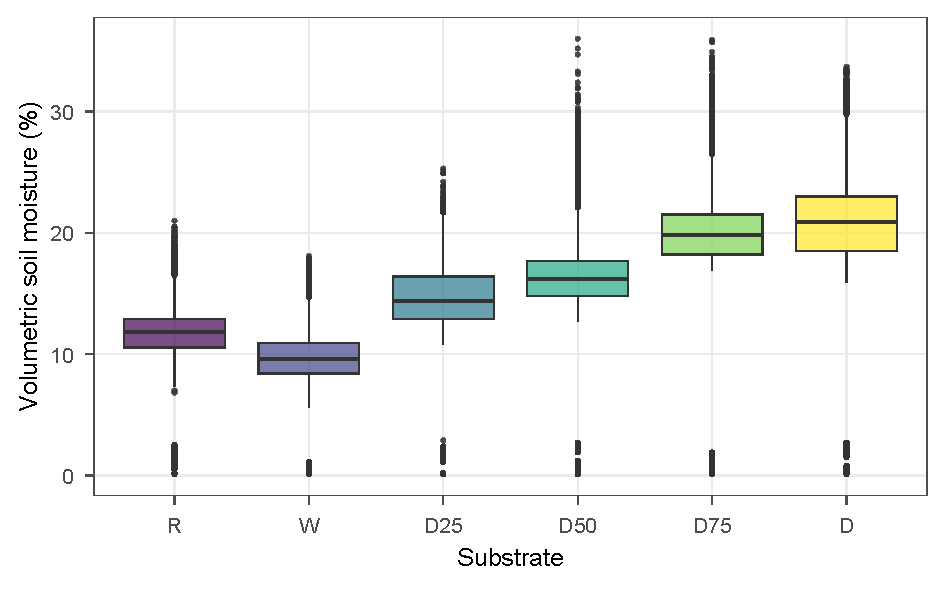
\includegraphics[width=\textwidth]{soil_moisture_boxplots.pdf}
        \caption{Soil moisture variations}
        \label{fig:soil_moisture_sponge}
    \end{subfigure}
    \caption{Visualisation of the experimental substrate properties: (a) Total Organic Carbon (TOC) gradient across the 10 substrate mixtures, establishing the experimental conditions, and (b) observed soil moisture variations corroborating the ``sponge effect'' of increased organic matter.}
    \label{fig:substrate_characterization}
\end{figure}


\subsection{Vegetation Experiments}

\subsubsection{Common-Garden Growth Experiment}

A common-garden experiment was established at the port of Zeebrugge to quantify the effect of substrate type on marram grass (\textit{C. arenaria}) growth under uniform climatic conditions. Plant cuttings comprising 10--15 leaves, sourced from natural dunes at Zeebrugge, were planted in custom-designed boxes (10 $\times$ 10 cm horizontal, 40 cm deep) on 23 October 2023. The 10 substrates were distributed across 120 boxes using a randomised block design, with 12 replicates per substrate; 100 boxes were planted with marram grass and 20 were left as unplanted controls. The boxes were placed outdoors in the harbour, exposed to the maritime climate of the Belgian coast.

Growth was quantified through biweekly measurements of maximum leaf length and total number of living leaves (defined as leaves $>$\SI{5}{\centi\metre} with $>$\SI{20}{\percent} green tissue) from April through September 2024. During the initial measurement, \SI{27}{\percent} of cuttings were observed to have died during winter; these were replanted in April 2024. To simulate natural sand burial---essential for marram grass vigour \citep{disraeli1984effect}---boxes were manually overblown with \SI{1}{\centi\metre} of natural beach sand (R) on three occasions (24 May, 5 July, and 16 August 2024). Weeds were removed to ensure substrate purity. Treatment effects on leaf height and number of leaves were analysed using generalised linear mixed models fitted in R. For height, a Gaussian LMM (\texttt{lme4}) was fitted with substrate, orthogonal polynomial time (quadratic), and their interaction as fixed effects and plant identity as a random intercept; a likelihood-ratio test confirmed that the quadratic time trend significantly improved fit over a linear specification ($\chi^2 = 103.18$, $p < 2 \times 10^{-16}$). Leaf count, being discrete count data (mean $= 9.3$, variance $= 37.3$), was modelled with a Poisson GLMM (log link; \texttt{glmmTMB} package) using the same fixed-effects structure and a random intercept for plant identity; the Poisson distribution provided an adequate fit, as the plant-level random intercept accommodated any residual overdispersion. Estimated marginal means (EMMs) were computed on the response scale with the \texttt{emmeans} package and compared using FDR-adjusted pairwise contrasts; compact letter displays (CLD) were derived to summarise group membership. Model-predicted trajectories were plotted using the \texttt{ggeffects} package to ensure visual--statistical concordance.

\subsubsection{Germination Experiment}

A parallel germination experiment tested the capacity of marram grass seeds to establish on six substrates (R, W, D, and three D/W mixtures at 25/75, 50/50, and 75/25). Pipes (\SI{12.5}{\centi\metre} diameter, \SI{30}{\centi\metre} height) were filled with substrate to \SI{5}{\centi\metre} below the rim, and 10 marram seeds were placed on the surface and covered with \SI{1}{\centi\metre} of natural beach sand (R). The experiment comprised 16 replicates per substrate (96 pipes total), arranged in a randomised complete block design at the same outdoor location as the growth experiment. TMS-4 microclimate loggers were installed in one replicate of each substrate to record soil temperature, surface temperature, air temperature, and soil moisture at 15-minute intervals.

Germinated seedlings were counted on 24 May 2024 (1~month after setup), and maximum seedling length per pot was measured biweekly from May through September 2024. Pots were overblown with \SI{1}{\centi\metre} natural beach sand (R) on 5 July and 16 August 2024. Germination rates (proportion of 10 seeds germinated at $t_1$) were analysed using a binomial GLM; because the residual deviance exceeded the residual degrees of freedom (dispersion ratio $= 2.41$), a quasibinomial correction was applied to obtain valid standard errors and pairwise comparisons. EMMs on the probability scale and CLD groups were derived from the quasibinomial model using the \texttt{emmeans} package. Seedling count trajectories were modelled with a Poisson GLMM (log link; \texttt{glmmTMB}) with substrate, orthogonal polynomial time (quadratic), and their interaction as fixed effects and pot identity as a random intercept. The Poisson distribution provided an adequate fit, as the pot-level random intercept accommodated residual overdispersion.


\subsection{Derivation of SOM Response Curves for Model Parameterisation}
\label{sec:som_response_derivation}

To translate the experimental growth and mortality observations into continuous functions suitable for the Living Dunes demographic module, we derived dose--response curves relating normalised plant performance to substrate TOC content. For each response variable---maximum leaf height, maximum leaf count (stem density), root biomass, and mortality---individual measurements were normalised to the treatment mean of the reference beach sand (R), yielding substrate-specific multipliers.

The overall effect of substrate treatment on each response variable was first tested using a Kruskal--Wallis rank-sum test on the individual-level data ($n = 120$ for aboveground variables, $n = 228$ for root biomass). Due to the high within-treatment variance characteristic of individual-plant measurements in heterogeneous field conditions, the Gaussian response curves were fitted to treatment-level means (10 substrates) using weighted non-linear least squares with the Levenberg--Marquardt algorithm (\texttt{nlsLM} from the \texttt{minpack.lm} R package). Inverse-variance weights ($1/\text{SE}^2_j$) were assigned to each treatment mean, giving higher precision to treatments with less dispersion. This approach is standard for dose--response parameterisation when within-treatment variation exceeds the between-treatment signal \citep{ritz2015dose}.

Growth responses were modelled as Gaussian functions:
\begin{equation}
f_{\text{growth}}(\SOM) = b_0 + a \cdot \exp\left(-\frac{(\SOM - \mu)^2}{2\sigma^2}\right)
\label{eq:gaussian_som}
\end{equation}
where $b_0$ is the baseline multiplier, $a$ is the response amplitude, $\mu$ is the optimal SOM (\% TOC), and $\sigma$ is the standard deviation controlling the peak width. Parameters were bounded to physically interpretable ranges ($b_0 \in [0.5, 1.5]$, $a \in [0, 2]$, $\mu \in [0, 3]$, $\sigma \in [0.1, 3.0]$). Goodness-of-fit was assessed using weighted $R^2$ on the treatment means.

Mortality was modelled using a binomial generalised linear mixed model (GLMM; \texttt{glmmTMB} package) with SOM as a fixed effect and spatial block (column position in the common garden) as a random intercept, reflecting the experimental design:
\begin{equation}
\mathrm{logit}(P_{\mathrm{survival}}) = \beta_0 + \beta_1 \cdot \SOM + u_j, \quad u_j \sim \mathcal{N}(0, \sigma^2_u)
\label{eq:mortality_glmm}
\end{equation}
where $u_j$ is the random intercept for column $j$. Model adequacy was evaluated using McFadden pseudo-$R^2$.


\subsection{Modelling Biomorphogenic Feedbacks}

We simulated coupled aeolian--vegetation--geomorphological feedbacks using the Living Dunes model framework (a complete model description and release is planned for a separate publication). The model operates on a regular grid (here at \SI{0.2}{\metre} and \SI{1.0}{\metre} resolution) using an hourly time step for aeolian and soil moisture processes and a daily time step for vegetation dynamics. The core simulation loop integrates environmental forcing (wind, precipitation, temperature), soil moisture dynamics, aeolian sediment transport, geomorphological change, and vegetation growth and mortality. This section describes the model components relevant to the present study, emphasising the extensions developed for SOM representation.

\subsubsection{Aeolian Transport Framework}

The aeolian transport module computes sediment flux following a saturation-based framework. At each time step, the model calculates (a) a spatially varying wind field accounting for topographic steering, flow separation in the lee of dunes, and vegetation drag; (b) threshold shear velocity incorporating corrections for moisture, roughness, cohesion, and slope; (c) a saturated transport rate; and (d) the actual transport rate, which evolves toward saturation over a characteristic length scale.

The base threshold shear velocity $\ust$ is computed using the Shao and Lu formulation \citep{shao2000simple}, which explicitly accounts for interparticle cohesion:
\begin{equation}
\ust = \sqrt{A_N \left(\frac{\rho_s}{\rho_a}\, g \, d + \frac{\gamma}{\rho_a \, d}\right)}
\label{eq:shao_lu}
\end{equation}
where $A_N = 0.0123$ is a dimensionless coefficient, $\rho_s$ is the particle density (\SI{2650}{\kilo\gram\per\cubic\metre} for quartz), $\rho_a$ is the air density (\SI{1.225}{\kilo\gram\per\cubic\metre}), $g$ is gravitational acceleration (\SI{9.81}{\metre\per\second\squared}), $d$ is the nominal grain diameter (in metres), and $\gamma$ is the interparticle cohesion parameter (\si{\kilo\gram\per\second\squared}). For clean mineral sand, $\gamma$ defaults to $3 \times 10^{-4}$ \si{\kilo\gram\per\second\squared} following \citet{greeley1985wind}.

The saturated sand transport rate was computed following \citet{bagnold1941physics}:
\begin{equation}
Q_s = C \frac{\rho_a}{g}\, \usw^3
\label{eq:bagnold_transport}
\end{equation}
where $C = 1.5$ is the transport efficiency coefficient and $\usw$ is the surface shear velocity. The actual transport rate evolves toward saturation over a saturation length $L_{sat} = \SI{1.5}{\metre}$ using an advection scheme.

Soil moisture correction of the threshold follows the Van Rijn and Strypsteen formulation \citep{vanrijn2020}:
\begin{equation}
\ust^{(w)} = \ust^{(d)} \left(1 + 2\,\tanh\left(w_p\right)\right)
\label{eq:moisture_correction}
\end{equation}
where $\ust^{(d)}$ is the dry threshold, and $w_p$ is the gravimetric moisture content in percent.


\subsubsection{Soil Moisture Model}

The Living Dunes soil moisture module resolves a two-layer soil column comprising a surface layer (top \SI{30}{\milli\metre}) and a deep layer, with an additional aerodynamic skin layer (\SI{2}{\milli\metre}) at the surface. The model is driven by hourly precipitation, temperature, and wind speed inputs, and computes potential evapotranspiration using the FAO-56 Penman--Monteith equation \citep{allen1998crop}. Canopy interception, throughfall, infiltration, drainage, capillary rise, and plant water uptake are resolved sequentially at each time step. Infiltration is limited by the saturated hydraulic conductivity (\SI{200}{\milli\metre\per\hour} for beach sand). Drainage from the surface layer follows an exponential decay toward field capacity, while capillary rise from the deep layer to the surface layer is modelled as a function of the moisture gradient between layers. Finally, plant water uptake is determined by a stress--response function based on root-zone moisture relative to field capacity and the wilting point.

\subsubsection{Vegetation Module}

Living Dunes resolves vegetation dynamics at the species level using a demographic framework with distinct life phases (seed bank, juvenile, adult). For marram grass, growth is governed by a base rate modulated by environmental response functions for soil moisture, temperature, sand burial, erosion, and---as parameterised in this study---substrate SOM content, combined through a geometric mean interaction model. The environmental response functions are parameterised using cardinal response curves, Gaussian functions, and sigmoid functions derived from field observations and literature values.

Adult marram grass density growth follows:
\begin{equation}
\frac{d\,\rho_v}{d\,t} = r_{base} \times \left(\prod_{i=1}^{n}\, f_i(E_i)\right)^{1/n} \times g(\rho_v)
\label{eq:veg_growth}
\end{equation}
where $r_{base}$ is the base growth rate (\num{0.01} per day), $f_i(E_i)$ are the $n$ environmental response functions for driver $E_i$ (moisture, temperature, burial, erosion, SOM), and $g(\rho_v)$ is a density-dependent regulation term modelled as an inverse logistic function with midpoint at \SI{90}{\percent} cover. Height growth is similarly regulated and additionally responds to burial depth through a cardinal response function peaking at \SIrange{60}{200}{\milli\metre\per\day} burial rate, reflecting the species' characteristic stimulation by moderate sand accretion \citep{disraeli1984effect, huiskes1979ammophila}.

The SOM response functions enter the geometric mean as additional environmental factors $f_{\SOM}(\cdot)$ for density growth and height growth (\cref{eq:gaussian_som}), parameterised from the treatment-mean fits described in \cref{sec:som_response_derivation}. The derived parameters for the Living Dunes vegetation model are listed in \cref{tab:som_derived_parameters}, and the response curves are shown in \cref{fig:som_response_curves}.

Marram grass mortality is evaluated using a multi-driver framework where environmental stressors are combined through a maximum interaction model---the single most stressful condition determines the stress level at each time step. Mortality drivers include drought stress (moisture below a critical threshold), temperature extremes, excessive burial ($>$\SI{65}{\milli\metre\per\day}), and root exposure from erosion. As the mortality response to SOM was not significant in the experimental data (\cref{sec:results_som_curves}), no SOM-specific mortality modifier was implemented in the present simulations.

Lateral spread is modelled through a two-component kernel: a diffusive spread to immediately neighbouring cells and longer-range rhizome colonisation (L\'{e}vy walk), both modulated by the same environmental response functions but with distinct base rates and density-dependent regulation \citep{bonte2021biomorphogenic}.


\subsubsection{SOM Extensions to the Living Dunes Model}
\label{sec:som_extensions}

Three new process pathways were implemented to represent the effects of SOM on dune development. Together, these extensions enable the model to differentiate between substrates with varying organic matter content and to capture the emergent effects on long-term dune morphology.

\paragraph{Pathway 1: Dynamic Field Capacity --- The ``Sponge Effect''}

Soil organic matter increases the intra-aggregate porosity and specific surface area of sandy soils, thereby enhancing their water-holding capacity. This is implemented using a pedotransfer function (PTF) following \citet{saxton2006soil}:
\begin{equation}
\theta_{fc}^{(eff)} = \theta_{fc}^{(base)} + \alpha_{\SOM} \cdot \frac{\SOM}{100}
\label{eq:ptf}
\end{equation}
where $\theta_{fc}^{(eff)}$ is the dynamically adjusted volumetric field capacity, $\theta_{fc}^{(base)}$ is the baseline field capacity of the mineral sand matrix (\num{0.20} for the beach sand at the study site), $\SOM$ is the soil organic matter content in percent, and $\alpha_{\SOM}$ is a dimensionless sensitivity coefficient (default \num{0.7}, typical range 0.5--1.0 for coastal sands). The effective field capacity is capped at porosity minus \SI{0.01} to prevent physically unrealistic saturation. This PTF ensures that organic-rich substrates retain more moisture after drainage events, directly influencing both plant water availability and the aeolian moisture correction (\cref{eq:moisture_correction}).

\paragraph{Pathway 2: Dynamic Organic Cohesion}

Beyond the abiotic interparticle cohesion intrinsic to the mineral fraction, organic matter creates additional interparticle bonds through organic polymers, root exudates, fungal hyphae, and biological soil crusts \citep{zobeck2013soil}. This is represented by injecting a dynamic cohesion modifier upstream of the base threshold calculation (\cref{eq:shao_lu}):
\begin{equation}
\gamma_{eff} = \gamma_{base} + \beta_{\SOM} \cdot \SOM \cdot \left(1 - D\right)
\label{eq:organic_cohesion}
\end{equation}
where $\gamma_{eff}$ is the effective interparticle cohesion (\si{\kilo\gram\per\second\squared}), $\gamma_{base} = 3 \times 10^{-4}$ \si{\kilo\gram\per\second\squared} is the abiotic baseline, $\beta_{\SOM} = 0.006$ \si{\kilo\gram\per\second\squared} per percent SOM is a scaling coefficient derived from the non-linear bounds reported by \citet{zobeck2013soil}, and $D$ is a dimensionless disturbance index (0 = fully crusted, 1 = fully disturbed). The effective cohesion $\gamma_{eff}$ replaces $\gamma$ in \cref{eq:shao_lu}, producing a spatially varying threshold that is higher in organic-rich, undisturbed areas and lower in recently eroded zones.

\paragraph{Pathway 3: Disturbance Index Dynamics}

Biological soil crusts and organic cohesive bonds are vulnerable to mechanical disruption by saltating grains \citep{belnap1998vulnerability}. The model tracks a spatially varying disturbance index $D$ that decays exponentially toward zero (full recovery) and is reset toward one proportionally to erosion intensity:
\begin{equation}
D(t + \Delta t) = D(t) \cdot \exp\left(-k_{recov}\, \Delta t\right)
\label{eq:disturbance_decay}
\end{equation}
where $k_{recov} = 0.01$ \si{\per\day} is the recovery rate, corresponding to a half-life of approximately 69 days. When net erosion occurs in a grid cell, the disturbance index is instantaneously increased:
\begin{equation}
D_{new} = D_{old} + \left(1 - D_{old}\right) \cdot \min\left(\frac{|m_{erosion}|}{m_{ref}},\, 1\right)
\label{eq:disturbance_reset}
\end{equation}
where $m_{erosion}$ is the eroded sand mass (\si{\kilo\gram}) and $m_{ref} = \SI{1}{\kilo\gram}$ is a reference erosion mass for full disturbance. This formulation creates a dynamic feedback: erosion disrupts the crust, temporarily reducing organic cohesion and lowering the threshold for further erosion, while recovery in quiescent periods progressively restores the protective crust.


\subsection{Simulation Design}

\subsubsection{Reference Beach Scenario}

A reference beach scenario (no vegetation, no dune restoration) was configured as the counterfactual baseline. The simulation domain covers the existing beach profile at Ostend at \SI{1}{\metre} resolution, with the seaward boundary set at mean sea level and the landward boundary at the toe of the existing sea dike. The non-erodible layer was defined using a hybrid approach: the dike surface was treated as fully non-erodible, and the beach non-erodible level was set to the mean water table level (+\SI{2.5}{\metre} TAW), preventing deflation below the hydrological base. The simulation was forced with hourly ERA5 reanalysis wind data (gust-corrected and coastal-adjusted using the Global Wind Atlas), Open-Meteo precipitation and temperature records, and covered year 1 (September 2021 -- September 2022) of the intended 10-year reference period.

\subsubsection{Dune Restoration Scenarios}

Ten dune restoration scenarios were configured corresponding to the 10 experimental substrates. Each scenario starts from the same initial topography (a constructed dune mound of prescribed geometry placed on the existing beach) and is planted with marram grass at an initial cover density derived from typical restoration practice. The simulations use \SI{0.2}{\metre} grid resolution and an hourly time step, running for 3 years (26,280 hourly steps from September 2021 to September 2024).

For each substrate scenario, the sediment properties ($D_{50}$, $D_{90}$, bulk density) and SOM content were set according to the measured substrate properties (\cref{tab:substrate_properties}). The SOM-dependent model pathways described in \cref{sec:som_extensions} were activated for all dune restoration scenarios. Environmental forcing was identical across all scenarios, obtained from a hybrid pipeline combining ERA5 reanalysis (wind) and Open-Meteo (temperature, precipitation) data specific to the Ostend site coordinates. The Living Dunes default parameterisation for the Atlantic European bioregion was used for all remaining model settings, including the marram grass species parameters.

\subsubsection{Storm Erosion Assessment with XBeach}

After the 3-year dune growth simulation, the resulting dune profiles were used as input for storm erosion assessment using XBeach \citep{roelvink2009modelling}. For each of the 10 scenarios, the 3D dune profile computed by Living Dunes was extracted as the initial bathymetry for XBeach.

The storm boundary conditions (water level, wave height, wave period) were based on a design storm calibrated to the hindcast of Storm Corrie (January 2022), which produced significant wave heights exceeding \SI{4}{\metre} and elevated water levels at the study site. XBeach was configured to use the measured grain size distributions to set the $D_{50}$ and $D_{90}$ for each substrate scenario. Aboveground biomass properties, including height, stem diameter, stem density, and a drag coefficient ($C_d$) set to 1.0 following \citet{mendez2004estimation}, were derived directly from the marram grass cover density predicted by Living Dunes at year 3. Root cohesion was implemented as additional soil strength in the root zone, with the root depth calculated from the Living Dunes allometric relationship ($\sqrt{\rho_v} \times \SI{1.5}{\metre}$). The model's hydrodynamic and sediment transport formulations were calibrated to the Storm Corrie hindcast, setting parameters such as wave-skewness transport (\texttt{facua}), breaker parameter (\texttt{gamma}), maximum wave height-to-depth ratio (\texttt{gammax}), minimum wet depth (\texttt{eps}), critical avalanche slopes (\texttt{wetslp}/\texttt{dryslp}), and skewness/asymmetry factors (\texttt{facSk}/\texttt{facAs}). Sediment transport was computed using the default Soulsby--Van Rijn formulation, and the seaward bathymetry was extended using measured profiles from the BPNS.

\subsubsection{Post-Storm Recovery Simulation}

Following the XBeach storm simulation, the eroded dune profiles were used as the initial condition for a subsequent Living Dunes recovery simulation. This second Living Dunes phase tested the self-restoring capacity of the dune under each substrate scenario after storm damage, with the same environmental forcing and model parameterisation as the pre-storm growth phase. The vegetation state (cover density, height, root depth) was initialised from the surviving vegetation distribution after storm erosion, accounting for root exposure and burial.


\subsection{Analysis Metrics}

To comprehensively evaluate the performance of alternative sediments, the simulations output several key metrics documenting dune growth and resilience. Geomorphological development was quantified by extracting the total sand volume above the non-erodible layer integrated over the restoration footprint, as well as the maximum crest height along the cross-shore profile. Ecological establishment was assessed through the spatially averaged marram grass cover density at the end of each growing season. To evaluate nature-based resilience, we quantified the storm erosion volume during the XBeach storm simulation and the subsequent recovery rate, defined as the dune volume gain per year during the post-storm Living Dunes simulation. Furthermore, the underlying biomorphogenic processes were analysed using the aeolian transport activity (percentage of active time steps, mean rate, and direction) and a moisture retention index representing the time-averaged surface soil moisture, serving as a proxy for SOM-driven ecohydrological enhancement.


% =============================================================================
% 3. RESULTS
% =============================================================================
\section{Results}

\subsection{Vegetation Response to Alternative Substrates}

\subsubsection{Growth Experiment}
\label{sec:results_growth}

Marram grass growth was significantly influenced by substrate type. A Gaussian LMM with substrate, quadratic time, and their interaction as fixed effects and plant identity as a random intercept was fitted for leaf height; a Poisson GLMM (log link) with the same structure was fitted for leaf count. Estimated marginal means (EMMs) for height ranged from \SI{43.9}{\centi\metre} (R) to \SI{59.4}{\centi\metre} (D50), a difference of \SI{15.5}{\centi\metre}. FDR-adjusted pairwise comparisons revealed that the reference beach sand (R) supported significantly shorter plants than five alternative substrates: D25, D37.5, D50, D75, and D87.5 (all $p_{\mathrm{adj}} < 0.05$; compact letter display groups a vs.\ b; \cref{tab:aboveground_lmm}). Substrates W, D12.5, D62.5, and D shared an intermediate group (ab). The D/W mixtures with intermediate dark fraction (D37.5 and D50, corresponding to \SIrange{0.97}{1.21}{\percent} TOC) produced the tallest plants, consistent with the Gaussian optimum derived for the SOM response curves (\cref{sec:results_som_curves}).

The number of living leaves showed a significant substrate effect in the Poisson GLMM. EMMs for leaf count ranged from 6.8 (D12.5, group a) to 12.2 (D, group b), with intermediate substrates in a shared group (ab). The pure dark dredging substrate (D, \SI{2.16}{\percent} TOC) supported significantly more leaves than the lower-SOM substrates, indicating that tiller production responds positively to organic enrichment across the full experimental range (0.06--2.16\% TOC) without evidence of a decline at the upper end. This monotonically increasing pattern has implications for the SOM response curve parameterisation discussed in \cref{sec:results_som_curves}.

\begin{figure}[htbp]
    \centering
    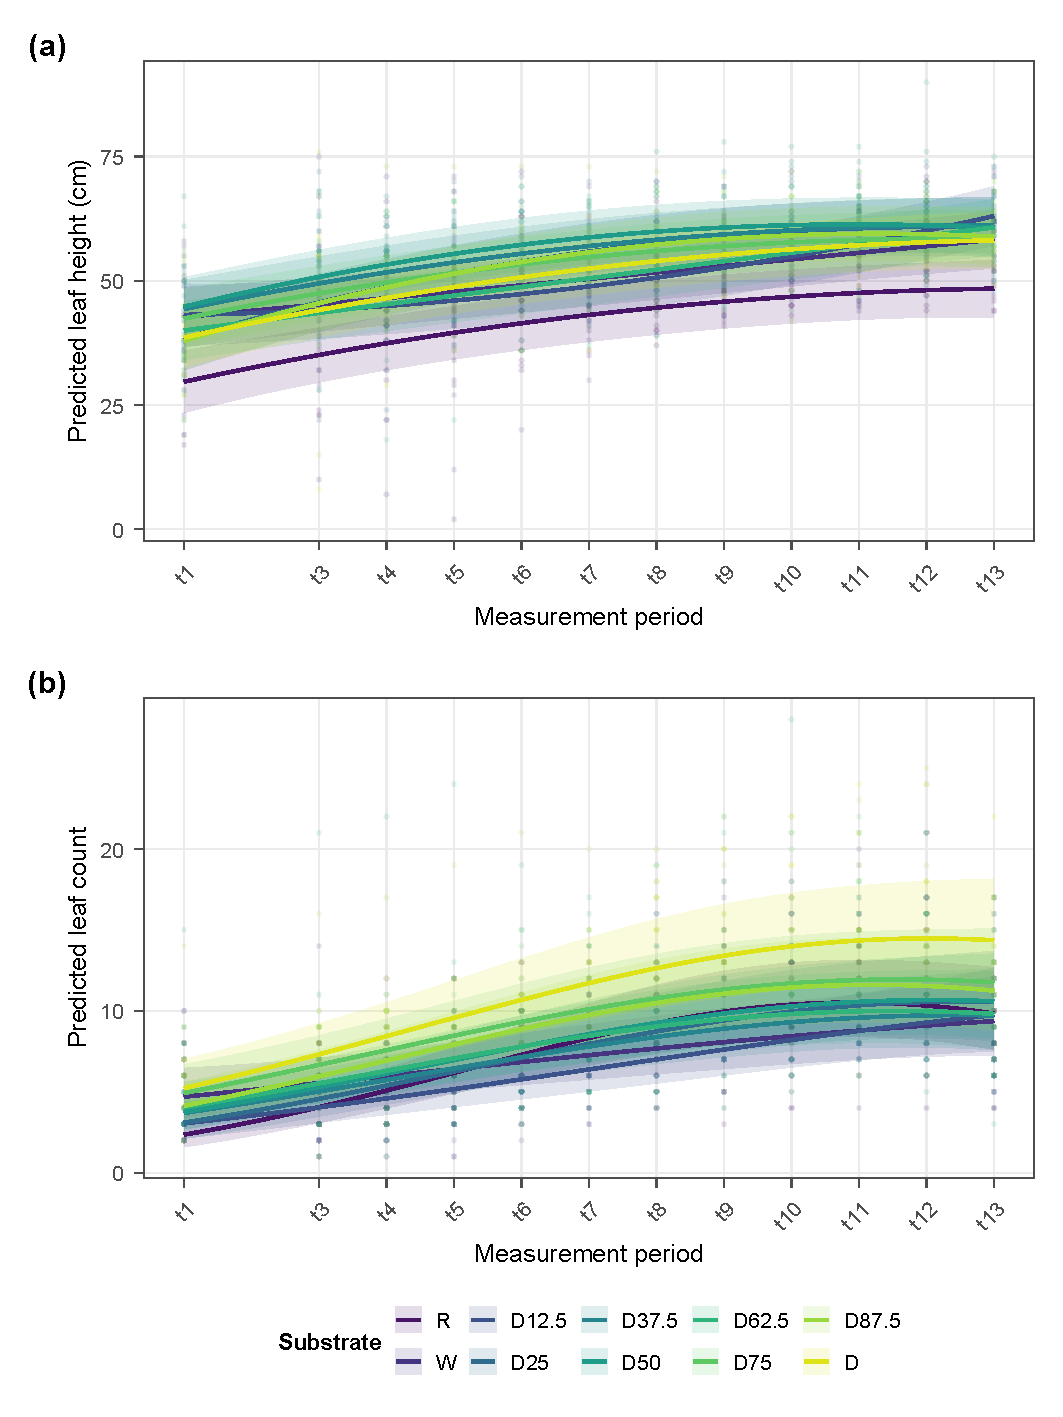
\includegraphics[width=\textwidth]{aboveground_growth_main.pdf}
    \caption{Aboveground growth trajectories during the common-garden experiment: (a) maximum leaf height and (b) number of living leaves over time, shown as model-predicted trajectories (Gaussian LMM and Poisson GLMM, respectively) with 95\% confidence bands. Raw data are plotted as semi-transparent points. Intermediate D/W mixtures produced optimal height; the pure dark sediment (D) supported significantly more leaves (group b) than the lower-SOM substrates. For full distributions and detailed boxplots, see \cref{sec:appendix_figures}.}
    \label{fig:aboveground_growth}
\end{figure}

\subsubsection{Germination Experiment}

Germination success differed strongly among substrates (quasibinomial GLM: $F(5, 90) = 13.01$, $p < 0.001$; dispersion ratio $= 2.41$). The reference beach sand (R) had the lowest germination probability (\SI{6.3}{\percent}, group a), followed by the pure dark substrate (D, \SI{23.1}{\percent}, group b), while the four intermediate substrates showed similarly high germination: W (\SI{53.1}{\percent}), D25 (\SI{46.9}{\percent}), D50 (\SI{49.4}{\percent}), and D75 (\SI{54.4}{\percent}; all group c). The low germination on R is consistent with observed seed loss through wind erosion on the bare, cohesionless sand surface, whereas the reduced performance on pure D may reflect surface crusting impeding seedling emergence.

Seedling establishment was modelled with a Poisson GLMM (seedling count $\sim$ substrate $\times$ polynomial time, random intercept per pot). Estimated marginal means (EMMs) revealed three compact letter display groups (\cref{tab:germination_stats}): R (group a, EMM $= 0.42$ seedlings), D (group b, EMM $= 2.25$), and W/D25/D50 (group bc, EMM $= 3.4$--$4.0$), with D75 performing best (group c, EMM $= 4.68$), confirming that seedling survival and growth were substrate-dependent beyond the initial germination differences.

The TMS-4 microclimate loggers revealed systematic differences in volumetric soil moisture consistent with the SOM gradient (Kruskal--Wallis: $\chi^2(5) = 634.92$, $p < 2 \times 10^{-16}$): moisture content increased from \SI{9.1}{\percent} (W) and \SI{10.8}{\percent} (R) to \SI{19.2}{\percent} (D), corroborating the pedotransfer-predicted ``sponge effect'' (\cref{tab:microclimate}). Soil temperature did not differ significantly among substrates ($\chi^2(5) = 1.23$, $p = 0.94$; all daily means within \SIrange{18.4}{18.8}{\degreeCelsius}), indicating that thermal conditions were uniform across treatments.

\begin{figure}[htbp]
    \centering
    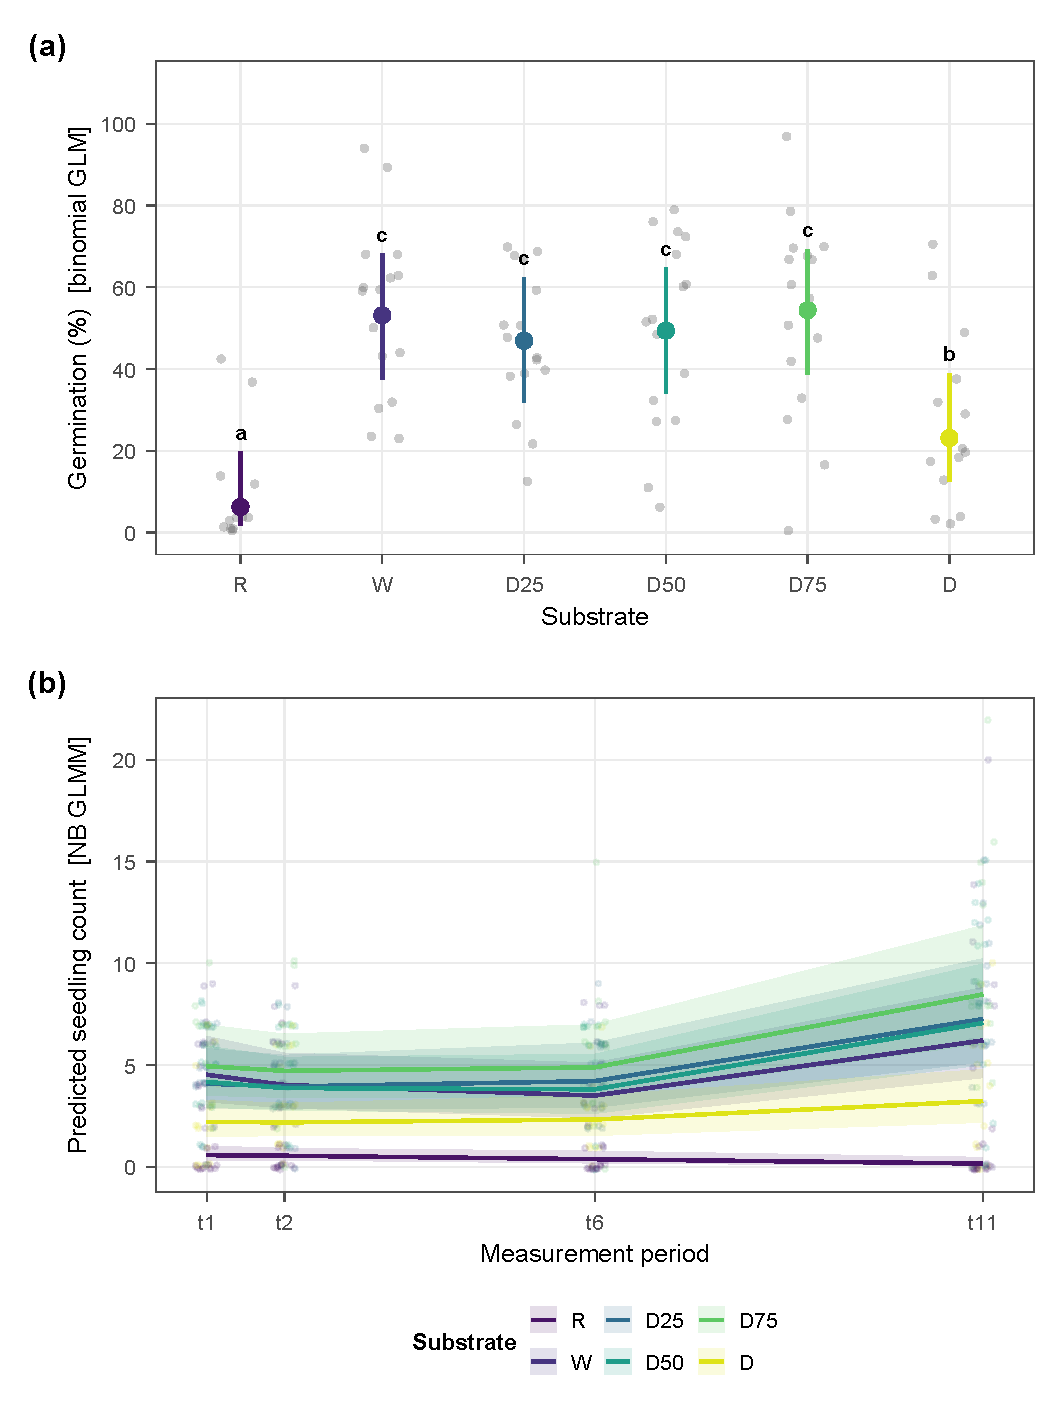
\includegraphics[width=\textwidth]{germination_main.pdf}
    \caption{Germination experiment results: (a) germination probability at $t_1$ across the six substrates estimated from the quasibinomial GLM and (b) seedling count over time showing model-predicted trajectories (Poisson GLMM) with 95\% confidence bands. The reference beach sand (R, group a) and pure dark substrate (D, group b) performed significantly worse than the intermediate D/W mixtures (group c). Compact letter display groups from FDR-adjusted pairwise EMM contrasts are shown in panel (a).}
    \label{fig:germination_establishment}
\end{figure}


\subsection{SOM Response Curves for Model Parameterisation}
\label{sec:results_som_curves}

Kruskal--Wallis tests on individual-level data did not detect a statistically significant overall effect of substrate treatment on any growth metric (height: $\chi^2 = 9.18$, $p = 0.42$; density: $\chi^2 = 5.03$, $p = 0.83$; root biomass: $\chi^2 = 5.17$, $p = 0.82$), owing to the large within-treatment variance among individual plants. However, the treatment-mean response patterns revealed biologically interpretable optima when fitted with Gaussian dose--response curves (\cref{fig:som_response_curves}).

Height growth showed a broad optimum centred at $\mu = 1.32$~\% TOC ($\sigma = 1.52$, amplitude $a = 0.81$; weighted $R^2 = 0.66$), indicating that substrates in the range 0.5--2.0~\% TOC marginally enhance vertical growth relative to pure beach sand, but without a sharply differentiated peak. Stem density growth yielded a Gaussian fit with a narrow optimum at $\mu = 0.65$~\% TOC ($\sigma = 0.10$, $a = 1.40$; weighted $R^2 = 0.64$); however, the fitted $\sigma$ reached the lower bound of the parameter space ($\sigma_{\min} = 0.10$), indicating that a Gaussian peak is a poor functional approximation for this trait. Indeed, the longitudinal Poisson GLMM in the growth experiment (\cref{sec:results_growth}) showed that leaf count increased monotonically across the full experimental SOM range to $2.16\%$ TOC, without evidence of a decline at higher SOM levels. The narrow Gaussian parameterisation should therefore be interpreted as a constrained fit imposed by the Living Dunes model's response function structure rather than a reflection of a true biological optimum at low SOM. Root biomass showed an intermediate pattern with an optimum at $\mu = 1.24$~\% TOC ($\sigma = 0.68$, $a = 0.65$; weighted $R^2 = 0.54$). Full coefficient tables are provided in \cref{sec:appendix_tables}.

The mortality GLMM revealed no significant SOM effect on survival probability ($\beta_1 = 0.010$, $p = 0.97$, McFadden pseudo-$R^2 \approx 0$), and negligible random-effect variance ($\sigma_u < 10^{-4}$). Across all substrates, approximately 20\% of transplanted marram grass individuals died, but this mortality was unrelated to organic matter content within the experimental range (0.06--2.16~\% TOC).

The derived response parameters are summarised in \cref{tab:som_derived_parameters}.

\begin{table}[htbp]
\centering
\caption{Derived SOM response parameters for the Living Dunes vegetation model. Growth responses use a Gaussian function as a multiplier on the base demographic rate. Mortality uses a sigmoid (inverse logistic) function. Density growth is excluded from the model parameterisation due to a single outlier driving the apparent response.}
\label{tab:som_derived_parameters}
\begin{tabular}{l l l r}
\toprule
Demographic process & Function & Parameter & Value \\
\midrule
Height growth & Gaussian & $\mu$ (\% TOC) & 1.323 \\
              &          & $\sigma$ (\% TOC) & 1.518 \\
              &          & Amplitude $a$ & 0.807 \\
\midrule
Density growth & --- & --- & Excluded$^\dagger$ \\
\midrule
Root growth & Gaussian & $\mu$ (\% TOC) & 1.242 \\
            &          & $\sigma$ (\% TOC) & 0.677 \\
            &          & Amplitude $a$ & 0.652 \\
\midrule
Mortality & Sigmoid & Steepness & -0.0105 \\
          &         & Threshold (\% TOC) & -126.21 \\
\bottomrule
\multicolumn{4}{l}{\footnotesize $\dagger$ One extreme measurement removed (plant 6b\_5, 97 leaves);} \\
\multicolumn{4}{l}{\footnotesize amplitude non-significant after removal ($p = 0.14$). See Table~\ref{tab:growth_coefficients}.} \\
\end{tabular}
\end{table}


\begin{figure}[htbp]
    \centering
    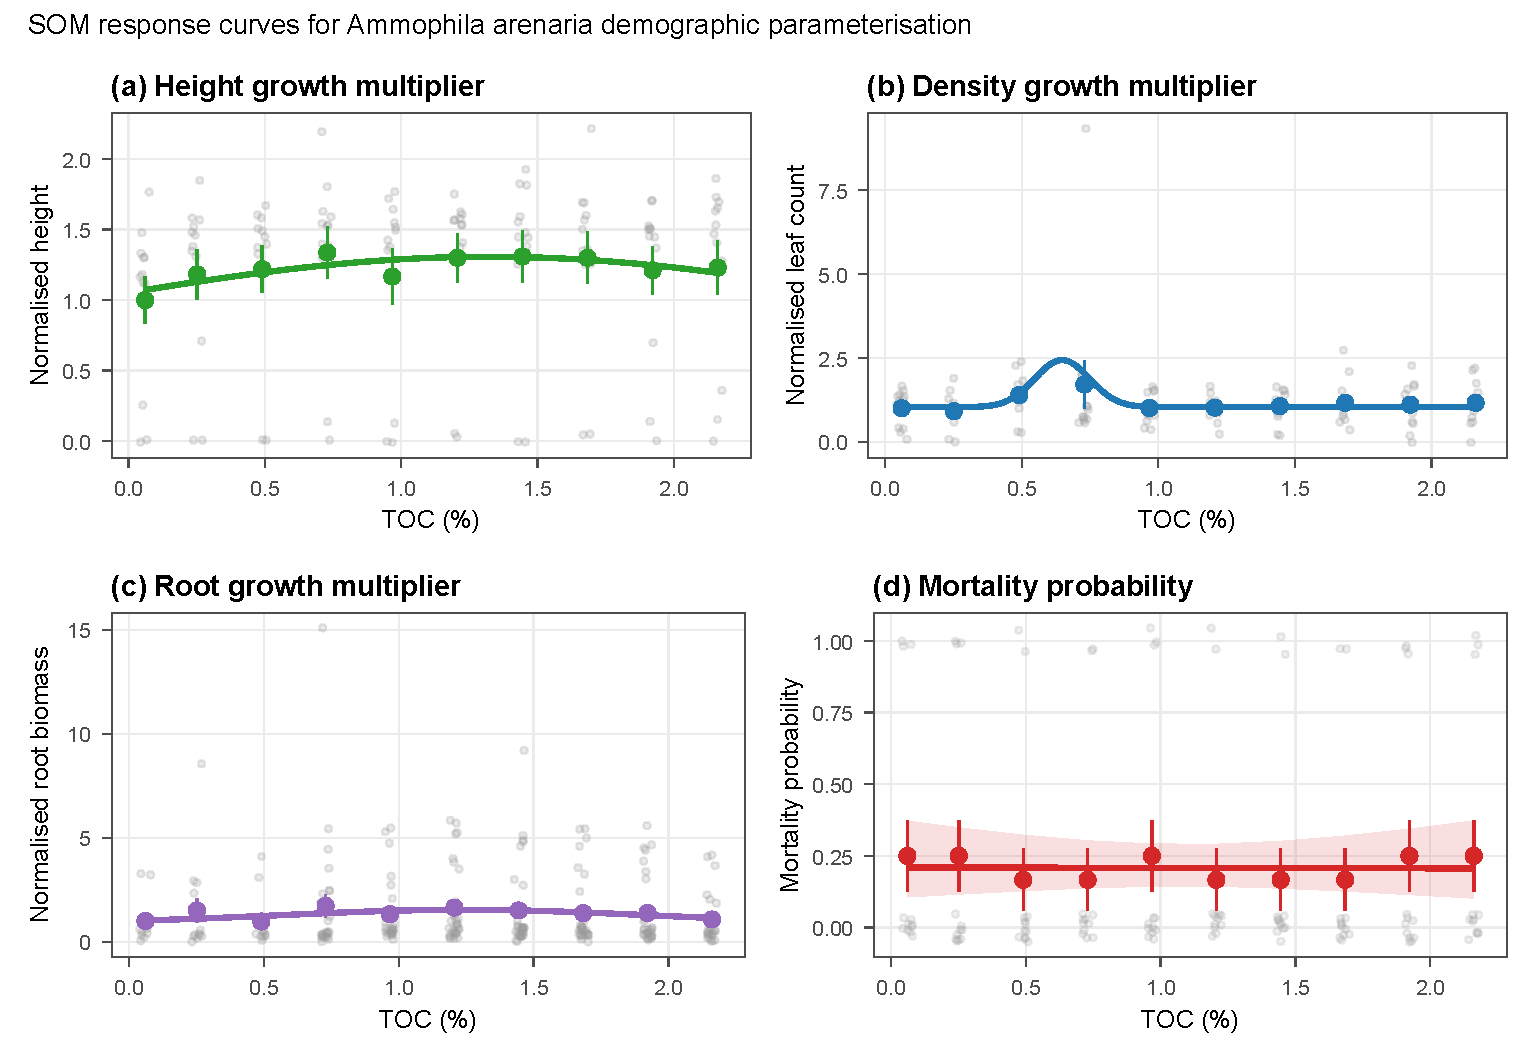
\includegraphics[width=\textwidth]{som_response_curves.pdf}
    \caption{SOM response curves for \textit{Ammophila arenaria} demographic parameterisation. Grey points show individual plant-level observations; coloured points with error bars show treatment means $\pm$ SE; solid lines show the fitted Gaussian (a--c) and logistic (d) curves. Mortality plots show the binomial GLMM marginal prediction with 95\% confidence band.}
    \label{fig:som_response_curves}
\end{figure}

\subsection{Reference Beach Simulation (Year 1)}

The reference beach simulation (no vegetation) produced results consistent with expected supply-limited beach dynamics. Over the first year (September 2021 -- September 2022), the beach zone experienced a net volume change of $-$\SI{362}{\cubic\metre}, comprising \SI{515}{\cubic\metre} of erosion and \SI{153}{\cubic\metre} of redeposition within the beach zone. The dike zone accumulated \SI{368}{\cubic\metre} of sand, representing aeolian deposition on and beyond the hard infrastructure.

Total aeolian influx was \SI{130}{\cubic\metre} and outflux was \SI{163}{\cubic\metre}, yielding a net aeolian flux balance of $-$\SI{33}{\cubic\metre}. Transport was active during \SI{2.4}{\percent} of the year (210 hours), with a mean gust-corrected wind speed of \SI{7.1}{\metre\per\second} (maximum \SI{25.0}{\metre\per\second}) and a dominant transport direction from the west (267\textdegree).


\subsection{Dune Development Under Different Substrate Scenarios}
\label{sec:dune_results}

\todo{Present 3-year dune development results for all 10 substrate scenarios once simulations are completed. Key results to report:
\begin{itemize}
    \item Cross-shore profile evolution over 3 years for each substrate;
    \item Dune volume accumulation curves;
    \item Vegetation cover density evolution;
    \item Effect of SOM on threshold shear velocity (spatial maps at year 3);
    \item Effect of SOM on soil moisture retention (temporal average);
    \item Optimal SOM range for dune growth (trade-off between enhanced vegetation and suppressed transport);
    \item Comparison of aeolian transport statistics across scenarios.
\end{itemize}
}


\subsection{Storm Erosion and Post-Storm Recovery}

\todo{Present XBeach storm erosion results and Living Dunes recovery simulation results for all 10 substrate scenarios once completed. Key results to report:
\begin{itemize}
    \item Pre-storm dune profiles (Living Dunes year 3) vs. post-storm profiles (XBeach);
    \item Erosion volume by substrate scenario;
    \item Role of root cohesion and vegetation drag in reducing storm erosion;
    \item Post-storm recovery trajectories (Living Dunes phase 2);
    \item Effect of substrate SOM on self-restoring capacity;
    \item Time to recover pre-storm dune volume.
\end{itemize}
}


% =============================================================================
% 4. DISCUSSION
% =============================================================================
\section{Discussion}

\subsection{SOM as a Double-Edged Sword for Dune Development}

The combined experimental and modelling results reveal that soil organic matter content acts as a ``double-edged sword'' for dune development in nature-based restoration settings. On one hand, SOM enhances vegetation establishment and growth through multiple mechanisms: higher germination rates due to increased seed retention on cohesive surfaces, improved water availability through the pedotransfer-mediated ``sponge effect'' on field capacity \citep{saxton2006soil}, and greater nutrient availability (both TOC and TN were positively correlated with plant performance). On the other hand, elevated SOM increases the threshold shear velocity through organic cohesion \citep{zobeck2013soil}, maintains higher surface moisture through enhanced water retention, and thereby progressively suppresses aeolian sediment supply---the very sand flux that marram grass depends on for continuous growth stimulation through burial \citep{huiskes1979ammophila, disraeli1984effect}.

This trade-off implies an optimal SOM range that maximises long-term dune development. Our growth experiments suggest that moderate D/W mixtures (50/50 and 37.5/62.5, corresponding to approximately \SIrange{1}{1.5}{\percent} TOC) produced the tallest marram grass, outperforming both the nutrient-poor reference sand and the excessively organic dark substrate. This bell-shaped response parallels the well-known ``optimal burial'' paradigm in dune ecology, where moderate sand accretion stimulates growth but excessive burial causes mortality \citep{maun1998adaptations}.

\subsection{SOM Influence on Marram Grass Demography}

The derived SOM response curves (\cref{sec:results_som_curves}) provide a nuanced picture of how substrate organic matter content influences individual demographic processes. Although the Kruskal--Wallis tests on individual-level data were non-significant---reflecting the large stochastic variation inherent in plant performance under heterogeneous field conditions---the treatment-mean curves revealed biologically interpretable optima consistent with the patterns observed in the raw growth data.

The height and root growth optima ($\mu = 1.32$ and $1.24$~\% TOC, respectively) were broad ($\sigma > 0.6$), indicating that these traits respond gradually to SOM enrichment within the experimental range. In contrast, the Gaussian fit for stem density growth converged to a narrow optimum at $\mu = 0.65$~\% TOC ($\sigma = 0.10$), although this narrow width should be interpreted cautiously: the fitted $\sigma$ reached the lower parameter bound, and the longitudinal Poisson GLMM showed a monotonically increasing leaf count trend across all tested SOM levels. The Gaussian form may underestimate the true density response at higher SOM values within the experimental range. This has implications for the Living Dunes model: because growth processes are combined through a geometric mean interaction (\cref{eq:veg_growth}), the narrowest response function effectively constrains the overall growth multiplier at extreme SOM values, even when other traits remain at or above baseline. Future work should evaluate alternative functional forms (e.g., saturating or log-linear curves) for the density response.

The absence of a significant SOM--mortality relationship within the experimental range (0.06--2.16~\% TOC) is a meaningful finding in itself: it indicates that, at least during the establishment phase, the organic matter levels tested do not induce phytotoxicity, anaerobic root conditions, or pathogen pressure sufficient to elevate mortality above the background rate of approximately 20\%. This result justifies omitting SOM from the mortality interaction model in the current simulations, although longer-term monitoring at higher SOM concentrations (where anaerobic conditions may develop) could reveal a mortality signal.

\subsection{Model Performance and SOM Pathway Interactions}

The three SOM integration pathways implemented in the Living Dunes model---the Saxton and Rawls pedotransfer function for dynamic field capacity, the Zobeck-based dynamic organic cohesion, and the Belnap and Gillette disturbance index---interact through positive and negative feedbacks that create emergent behaviour not predictable from any single pathway in isolation. The experimentally derived SOM growth curves (\cref{tab:som_derived_parameters}) add a fourth interaction: the direct demographic effect of substrate quality on marram grass vigour, which modulates the vegetation--aeolian feedback independently of the physical SOM pathways.

The positive feedback operates as follows: SOM increases moisture retention (Pathway 1), which enhances vegetation growth (\cref{eq:veg_growth} via the moisture response function), which in turn produces more litter and root exudates that further increase SOM. Simultaneously, the vegetation canopy reduces surface wind shear through aerodynamic roughness, allowing the disturbance index to decay toward zero (Pathway 3), which maximises the organic cohesion contribution (Pathway 2), further reducing erosion. The demographic SOM response amplifies this cascade: at moderate SOM levels ($\sim$1~\% TOC), the Gaussian growth multiplier exceeds unity, further boosting vegetation cover beyond what moisture alone would predict.

The negative feedback acts in opposition: as SOM increases threshold shear velocity (Pathway 2) and surface moisture (Pathway 1), aeolian sand supply to the dune crest diminishes. Without fresh sand burial, marram grass vigour declines \citep{vanderputten1993plant}, growth rates decrease, and mortality may increase, ultimately reducing vegetation cover and organic matter input. This negative feedback prevents runaway stabilisation and maintains the dynamic equilibrium between vegetation and aeolian processes that characterises natural dune systems.

The balance between these feedbacks depends critically on the SOM content and the local wind climate. Under the moderate wind regime of the Belgian coast (mean gust-corrected speed \SI{7.1}{\metre\per\second}), the negative feedback is expected to become dominant at the higher end of the experimental SOM range ($\sim$\SI{2}{\percent} TOC), where the combined effects of enhanced moisture retention and organic cohesion substantially increase the threshold shear velocity, suppressing transport during all but the most energetic events.

\subsection{Implications for Practice}

The experimental and modelling results converge on several practical recommendations for the use of alternative sediments in DfD construction:

First, moderate mixing ratios (\SIrange{25}{50}{\percent} dark dredging material in a white dredging or beach sand matrix) appear to optimise the trade-off between vegetation establishment and aeolian dynamics. Pure dredging material, while beneficial for initial plant establishment, may suppress the aeolian sand supply necessary for long-term dune growth.

Second, the placement geometry of the alternative substrate matters. Our model resolves the spatial distribution of SOM and its effects on threshold shear velocity, suggesting that a stratified approach---placing organic-rich material at the core of the constructed dune for moisture retention, overlain by a thinner cap of natural sand that preserves aeolian mobility---may outperform homogeneous mixing.

Third, the self-restoring capacity of the dune after storm erosion depends on the substrate: dunes built with moderate SOM are expected to recover faster because surviving vegetation benefits from enhanced moisture and nutrient availability during the critical post-storm recolonisation phase, while the exposed organic-rich core provides immediate germination substrate for natural recruitment.

\subsection{Limitations and Future Work}

Several limitations should be acknowledged. The growth experiments covered a single growing season; longer-term monitoring is needed to assess whether the initial substrate advantage persists as the dune surface becomes covered with fresh aeolian sand. The Living Dunes model currently represents SOM as a static property initialised at the start of the simulation; a fully dynamic SOM cycle---including litter production, decomposition, bioturbation, and aeolian redistribution of organic particles---is under development but was not activated in the present simulations. The SOM-to-cohesion scaling coefficient ($\beta_{\SOM} = 0.006$ \si{\kilo\gram\per\second\squared} per \% SOM) is derived from wind tunnel studies on agricultural soils \citep{zobeck2013soil} and may differ for coastal dune substrates; site-specific wind tunnel validation is recommended.

The XBeach storm modelling component uses simplified representations of root cohesion and vegetation drag that do not fully resolve the three-dimensional root network architecture. Furthermore, the coupling between Living Dunes and XBeach is currently one-directional (Living Dunes provides initial conditions to XBeach); a bidirectional coupling that feeds storm impact back into the aeolian--vegetation feedback loop in real time would enable more realistic long-term projections.

Future work should include (i) multi-year field monitoring of DfD sites constructed with alternative sediments, (ii) wind tunnel experiments quantifying the threshold shear velocity of dredging substrates with varying organic content, (iii) extension of the model to include dynamic SOM cycling, and (iv) application to other NBS sites along the North Sea coast where alternative sediment use is being considered.


% =============================================================================
% 5. CONCLUSION
% =============================================================================
\section{Conclusion}

This study demonstrates that soil organic matter content is a first-order control on dune development in nature-based coastal restoration settings, operating through three mechanistic pathways: enhanced soil water retention, increased threshold shear velocity via organic cohesion, and nutrient-mediated vegetation performance. Common-garden experiments confirmed that marram grass establishes and grows significantly better on organic-rich alternative substrates from port dredging than on natural beach sand, with the strongest effects observed during the critical establishment phase. The Living Dunes model, extended with pedotransfer-based dynamic field capacity, organic cohesion dynamics, and a disturbance recovery index, successfully captures the emergent trade-off between vegetation vigour and aeolian sand supply that governs dune morphological development.

Simulations of 10 substrate scenarios at Ostend indicate that moderate SOM enrichment (\SIrange{1}{2}{\percent} TOC) optimises long-term dune development by simultaneously enhancing vegetation establishment and maintaining sufficient aeolian transport for continued dune growth. At the organic-rich end of the experimental range ($>$\SI{2}{\percent} TOC), the threshold shear velocity increase from enhanced moisture retention and organic cohesion begins to suppress aeolian sand supply, suggesting diminishing geomorphological returns despite continued ecological benefits.

These findings provide the first quantitative evidence-base for the use of dredging by-products in nature-based coastal defence, demonstrating that carefully selected mixing ratios of alternative sediments can enhance both the ecological and geomorphological performance of DfD systems. The integrated experimental--numerical framework presented here offers a transferable methodology for optimising sediment reuse in coastal restoration projects worldwide.


% =============================================================================
% ACKNOWLEDGEMENTS
% =============================================================================
\section*{Acknowledgements}

This work was supported by the SUSANA project (Sustainable Use of Sand in Nature-based Solutions). We thank the Flemish Maritime Services Division (MDK) for access to the study site and dredging material, and the port authority of Zeebrugge for hosting the field experiments. \todo{Complete acknowledgements.}


% =============================================================================
% REFERENCES
% =============================================================================

% Include references present in the list but not explicitly cited in the text
\nocite{davidson2005wind, devries2014aeolian, fecan1999parametrization, greeley1985wind}

\bibliographystyle{apalike}
\bibliography{references}

% Include the appendix
% =============================================================================
% SOM_dune_development_appendix.tex
% Appendix: Supplementary Figures and Tables
% =============================================================================

\clearpage
\appendix
\section{Supplementary Figures}
\label{sec:appendix_figures}

% --- Detailed Substrate Characterisation ---
\begin{figure}[htbp]
    \centering
    \begin{subfigure}[b]{0.85\textwidth}
        \centering
        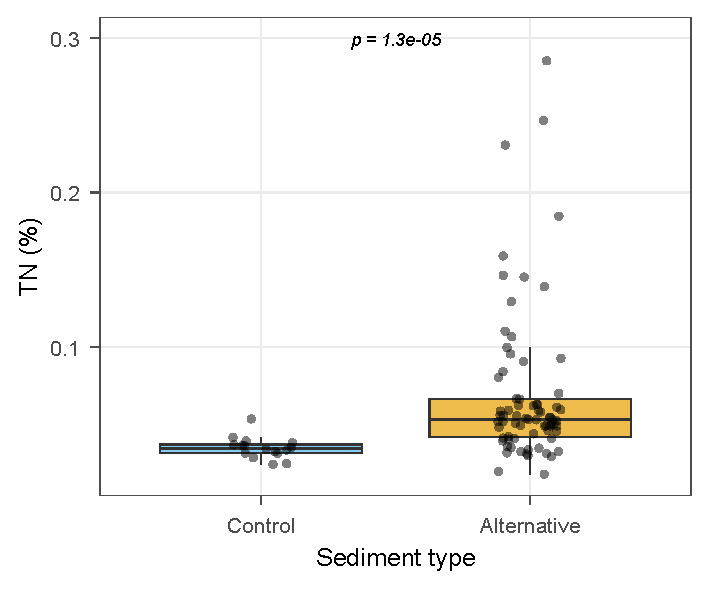
\includegraphics[width=\textwidth]{substrate_tn.pdf}
        \caption{Total nitrogen by substrate}
        \label{fig:app_substrate_tn}
    \end{subfigure}
    \par\vspace{1em}
    \begin{subfigure}[b]{0.85\textwidth}
        \centering
        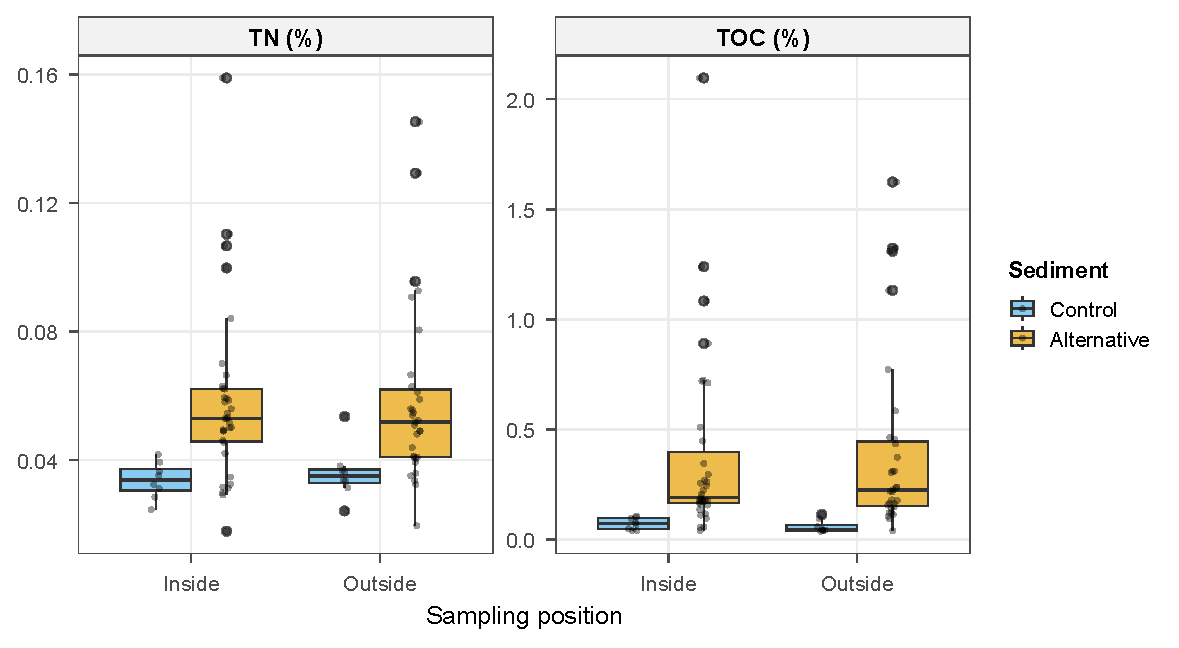
\includegraphics[width=\textwidth]{substrate_in_out_comparison.pdf}
        \caption{Inside vs.\ outside sampling comparison}
        \label{fig:app_substrate_inout}
    \end{subfigure}
    \caption{Additional substrate characterisation: (a) Total nitrogen content across the 10 substrates, confirming the nutrient gradient, and (b) comparison of physical and chemical properties between inside- and outside-box sampling positions within the alternative substrates, validating spatial homogeneity ($p > 0.7$ for all Wilcoxon rank-sum tests; \cref{tab:substrate_stats}).}
    \label{fig:app_substrate_variance}
\end{figure}

% --- Detailed Aboveground Distributions ---
\begin{figure}[htbp]
    \centering
    \begin{subfigure}[b]{0.85\textwidth}
        \centering
        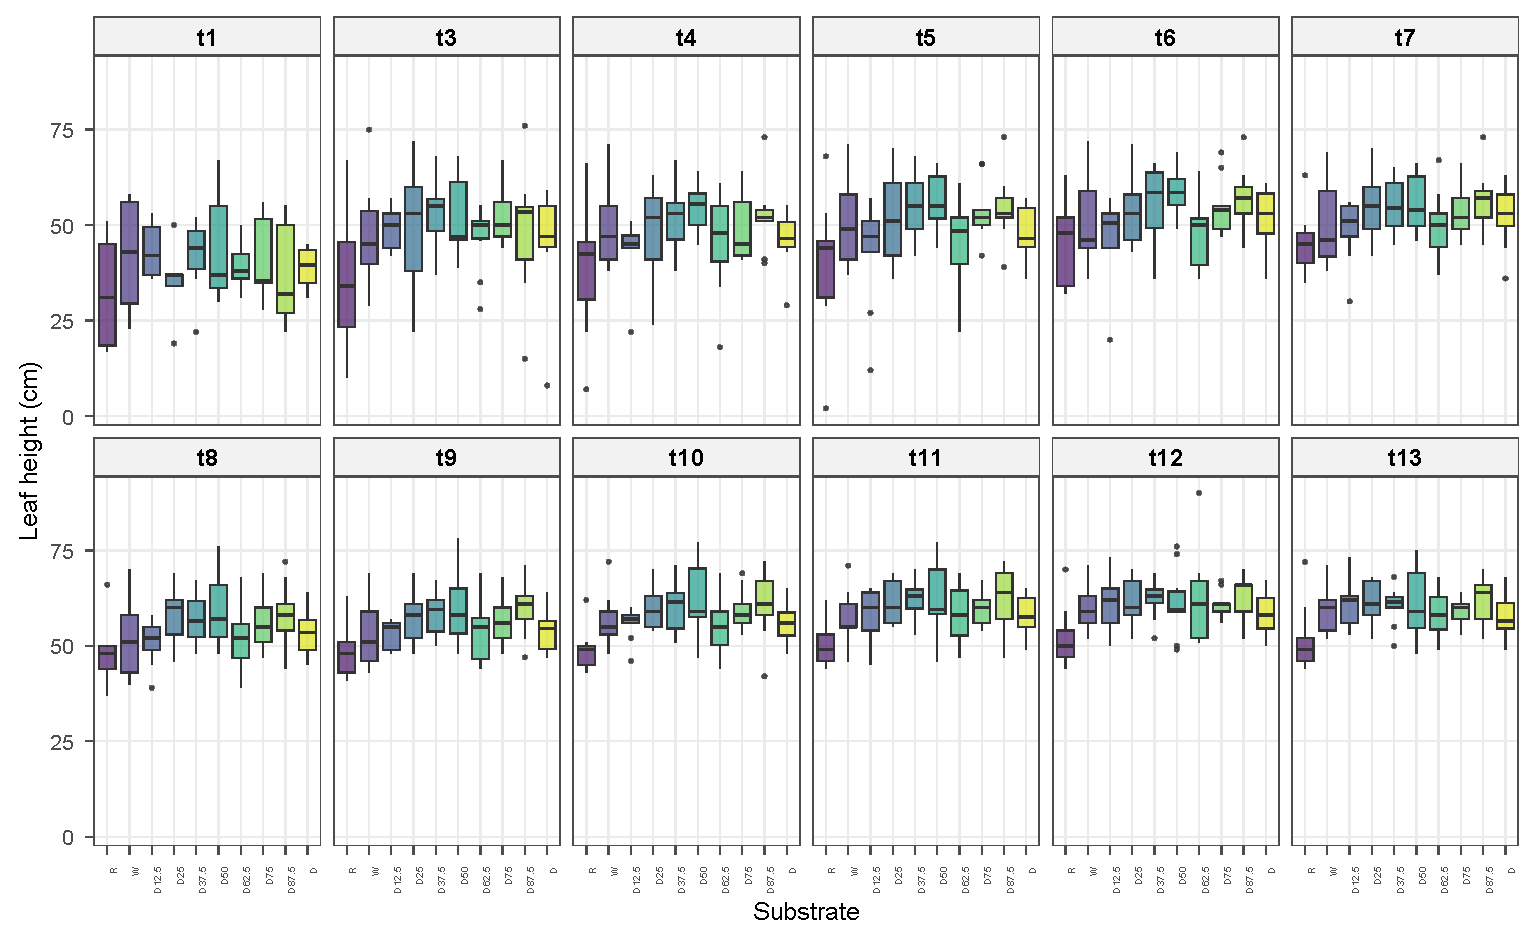
\includegraphics[width=\textwidth]{marram_height_all.pdf}
        \caption{Marram height distributions by time point}
        \label{fig:app_height_all}
    \end{subfigure}
    \par\vspace{1em}
    \begin{subfigure}[b]{0.85\textwidth}
        \centering
        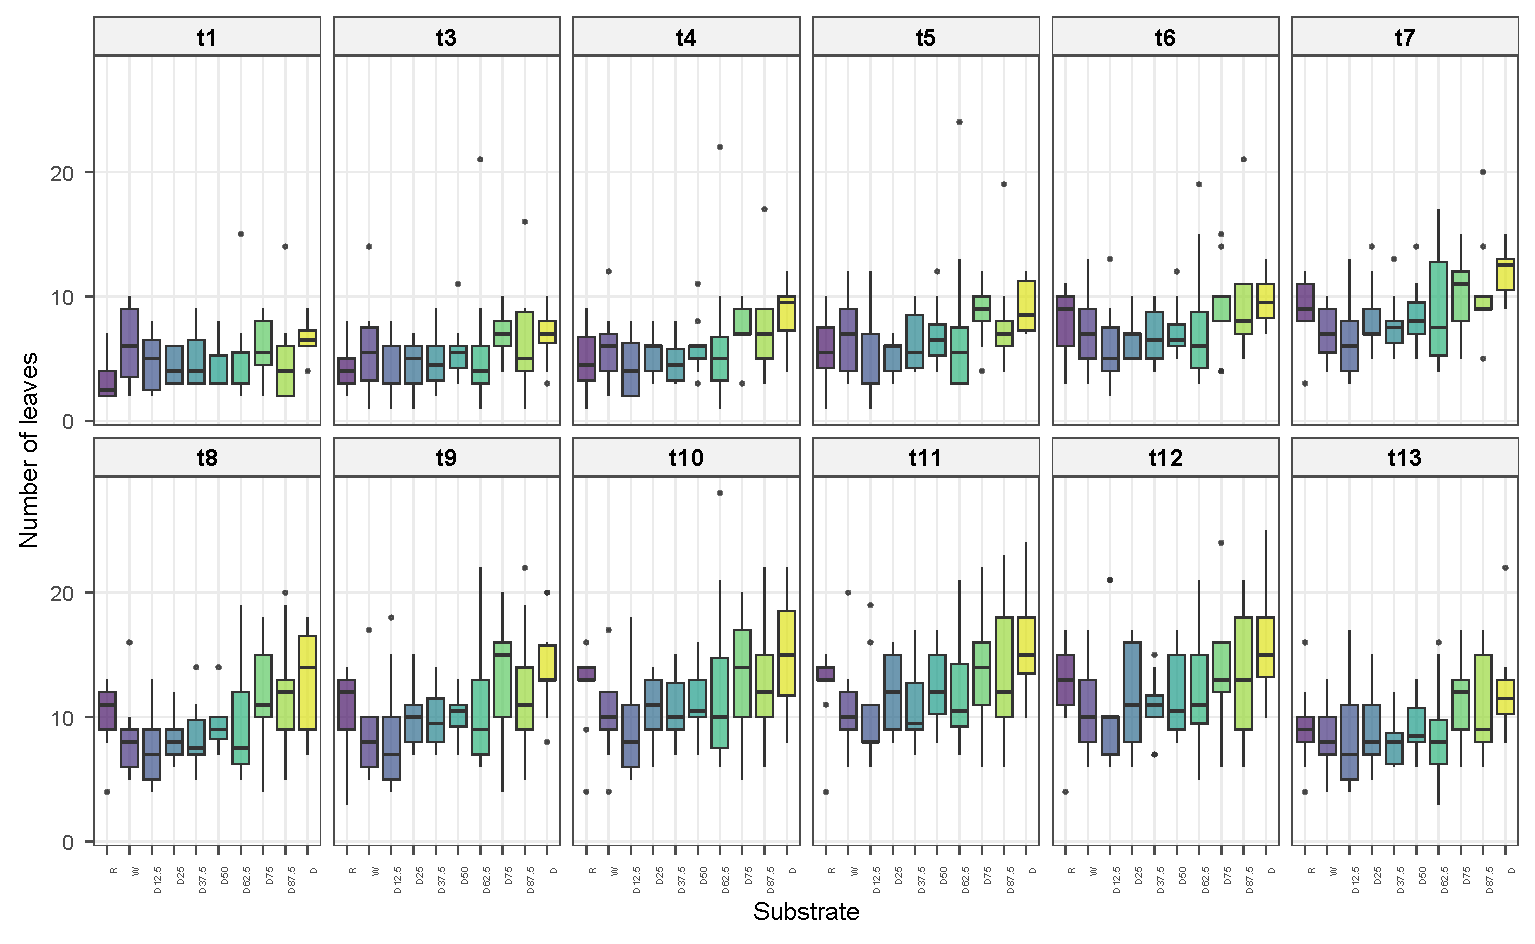
\includegraphics[width=\textwidth]{number_of_leaves.pdf}
        \caption{Leaf count distributions by time point}
        \label{fig:app_leaves_all}
    \end{subfigure}
    \caption{Detailed time-series boxplots of aboveground plant performance by substrate and measurement date. These non-parametric distributions underpin the model-predicted trajectories (Gaussian LMM for height, Poisson GLMM for leaf count) shown in the main text (\cref{fig:aboveground_growth}).}
    \label{fig:app_aboveground_dist}
\end{figure}

% --- Belowground Biomass ---
\begin{figure}[htbp]
    \centering
    \begin{subfigure}[b]{0.85\textwidth}
        \centering
        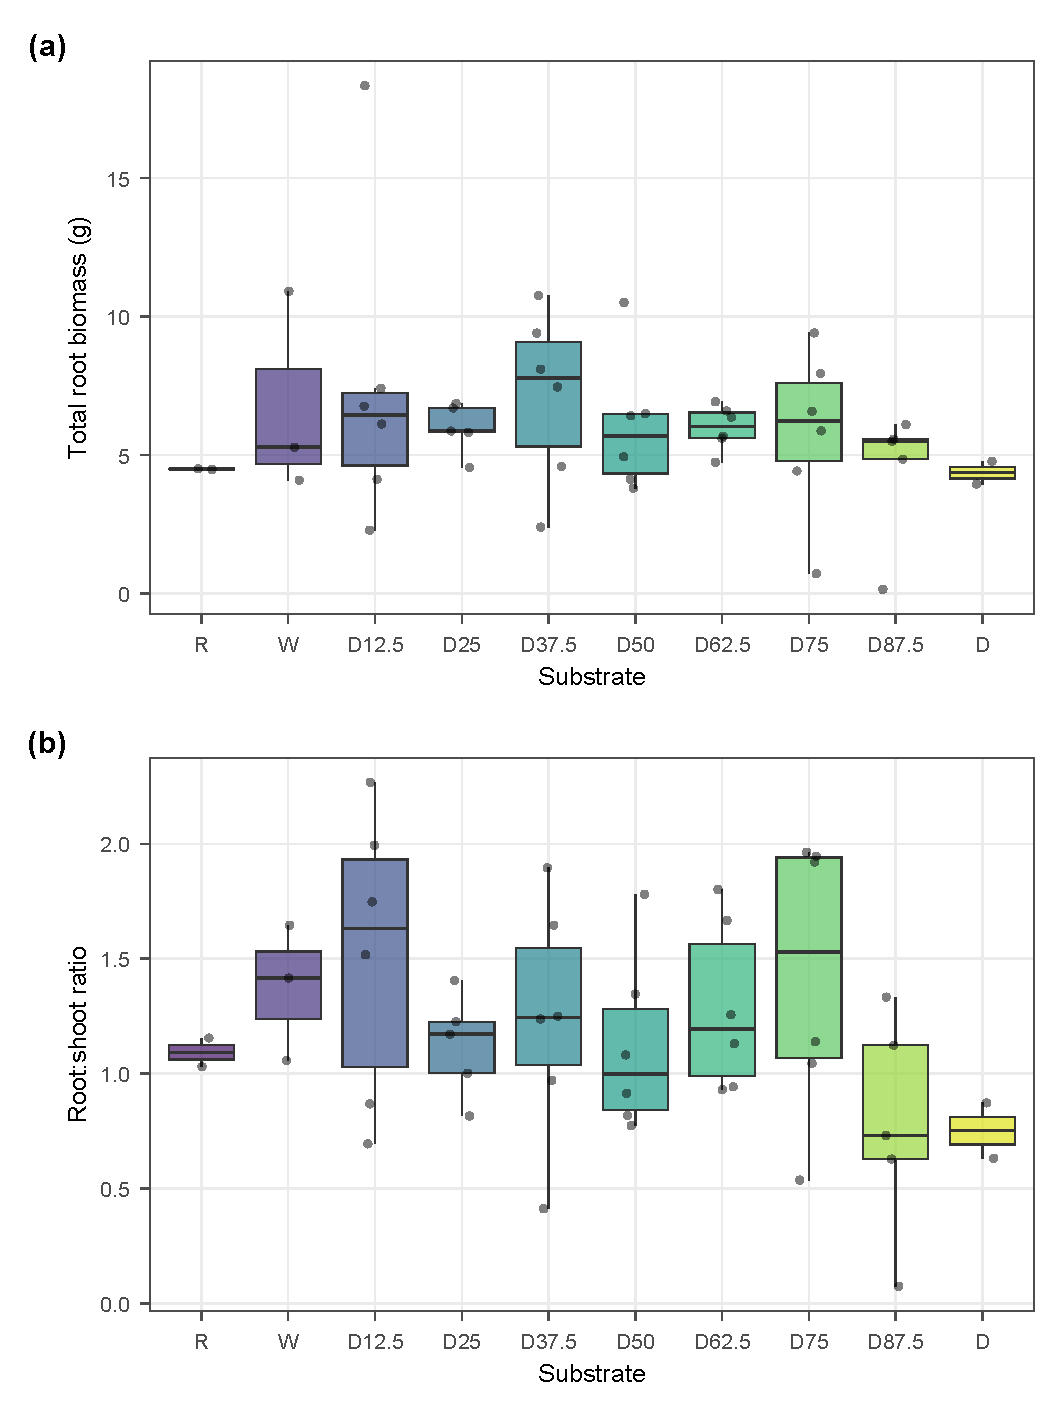
\includegraphics[width=\textwidth]{belowground_main.pdf}
        \caption{Root biomass and root:shoot ratio}
        \label{fig:app_root_shoot}
    \end{subfigure}
    \par\vspace{1em}
    \begin{subfigure}[b]{0.85\textwidth}
        \centering
        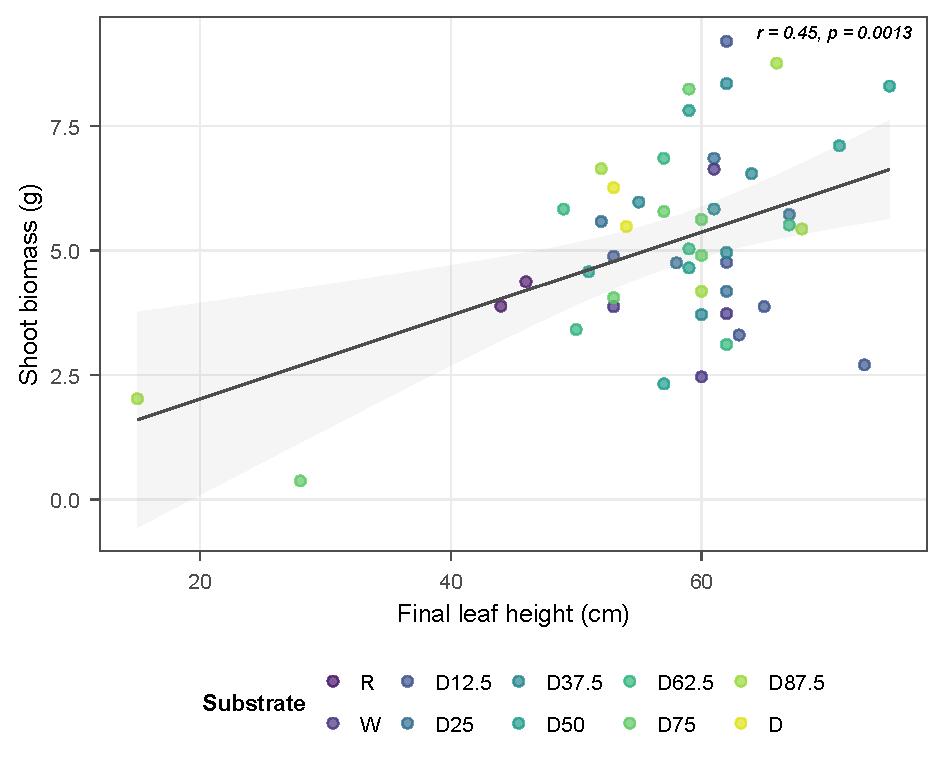
\includegraphics[width=\textwidth]{height_vs_shoot_biomass.pdf}
        \caption{Height vs.\ shoot biomass ($r = 0.45$, $p = 0.001$)}
        \label{fig:app_height_biomass}
    \end{subfigure}
    \par\vspace{1em}
    \begin{subfigure}[b]{0.85\textwidth}
        \centering
        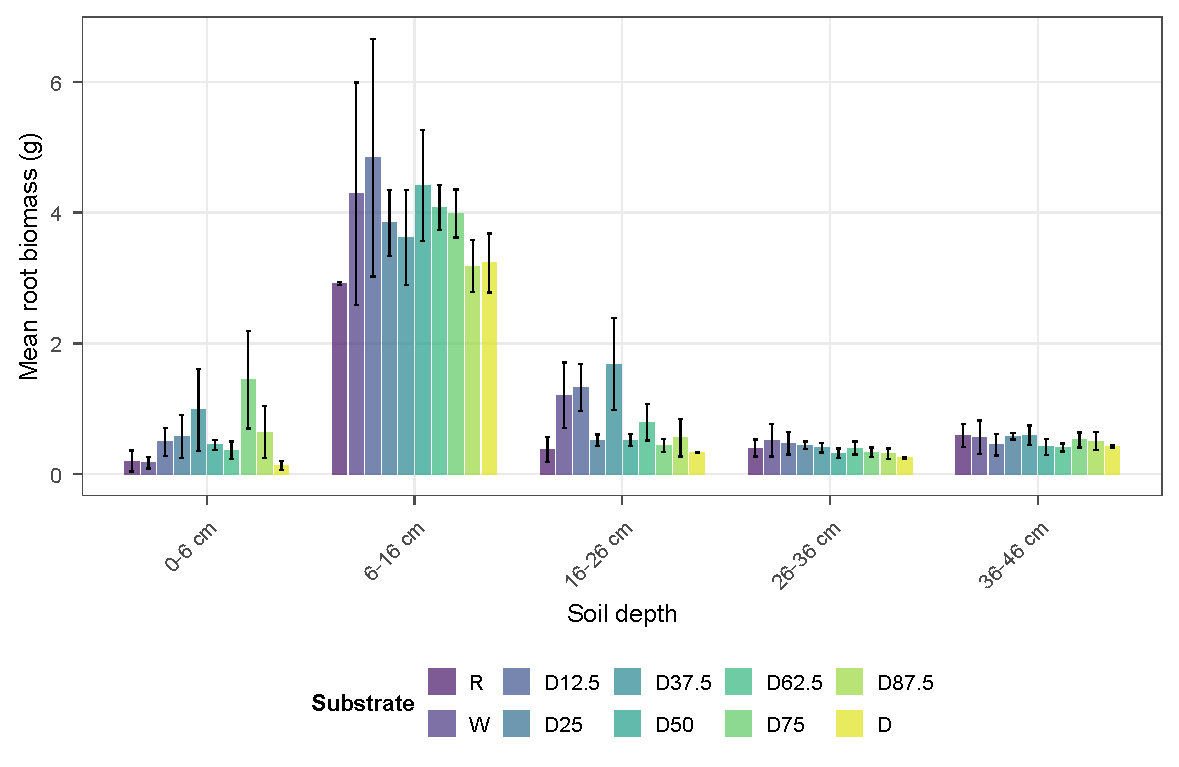
\includegraphics[width=\textwidth]{root_depth_profile.pdf}
        \caption{Root biomass depth profile}
        \label{fig:app_root_depth}
    \end{subfigure}
    \par\vspace{1em}
    \begin{subfigure}[b]{0.85\textwidth}
        \centering
        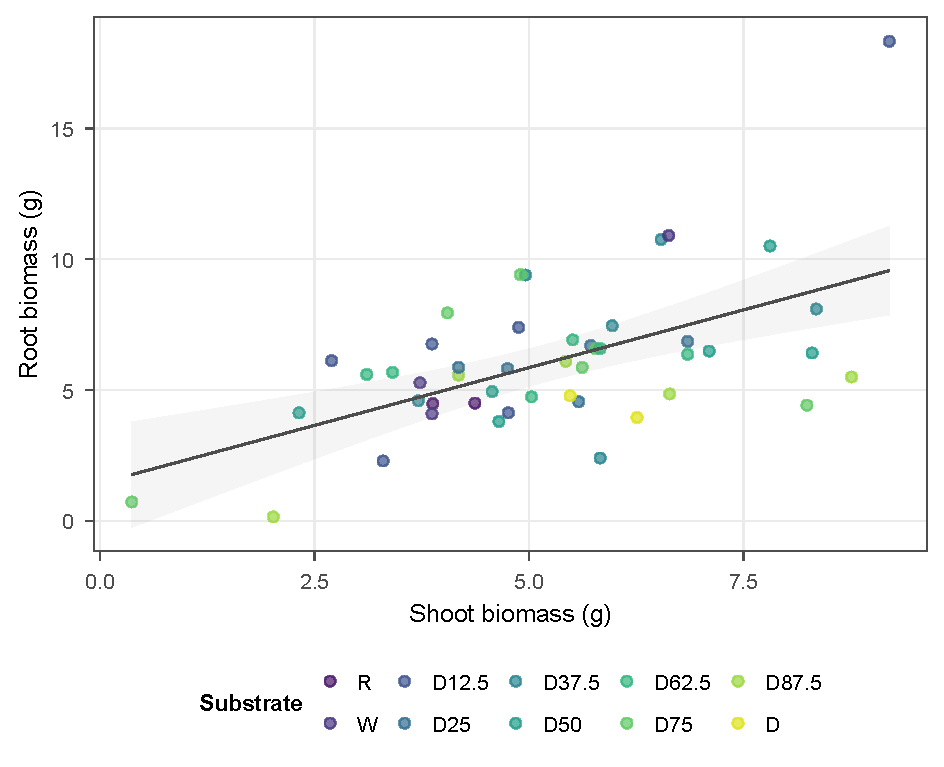
\includegraphics[width=\textwidth]{root_vs_shoot_scatter.pdf}
        \caption{Root vs.\ shoot biomass by substrate}
        \label{fig:app_root_vs_shoot}
    \end{subfigure}
    \caption{Belowground biomass allocation. No significant substrate effects were detected by either Gamma GLMs or Kruskal--Wallis tests for total root biomass ($F = 0.68$, $p = 0.72$; $\chi^2 = 6.87$, $p = 0.65$), root:shoot ratio ($F = 1.41$, $p = 0.22$; $\chi^2 = 9.67$, $p = 0.38$), or shoot biomass ($F = 0.43$, $p = 0.91$; $\chi^2 = 5.76$, $p = 0.76$). Height was significantly positively correlated with shoot biomass (b), confirming the allometric relationship used in the Living Dunes vegetation model.}
    \label{fig:app_belowground}
\end{figure}

% --- Detailed Microclimate Data ---
\begin{figure}[htbp]
    \centering
    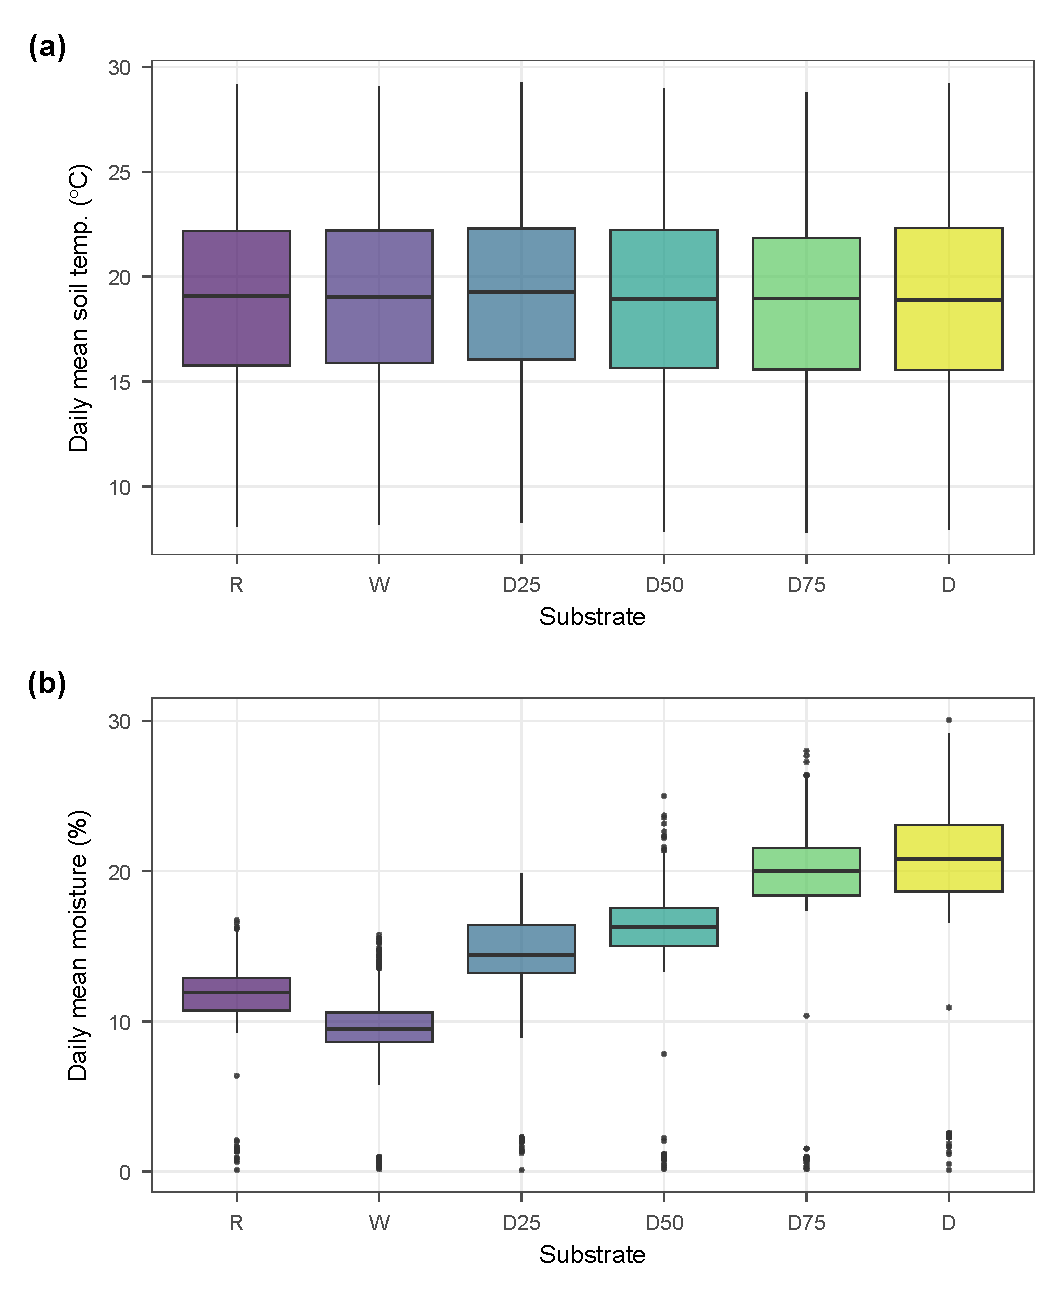
\includegraphics[width=0.85\textwidth]{microclimate_boxplots.pdf}
    \caption{Overview of microclimate variables recorded by TMS-4 loggers during the germination experiment ($\sim$225 days). Soil temperature did not differ significantly among substrates ($\chi^2(5) = 1.23$, $p = 0.94$; Kruskal--Wallis), while volumetric soil moisture showed a clear SOM gradient ($\chi^2(5) = 634.92$, $p < 2 \times 10^{-16}$; Kruskal--Wallis).}
    \label{fig:app_clim_vars}
\end{figure}

\begin{figure}[htbp]
    \centering
    \begin{subfigure}[b]{0.85\textwidth}
        \centering
        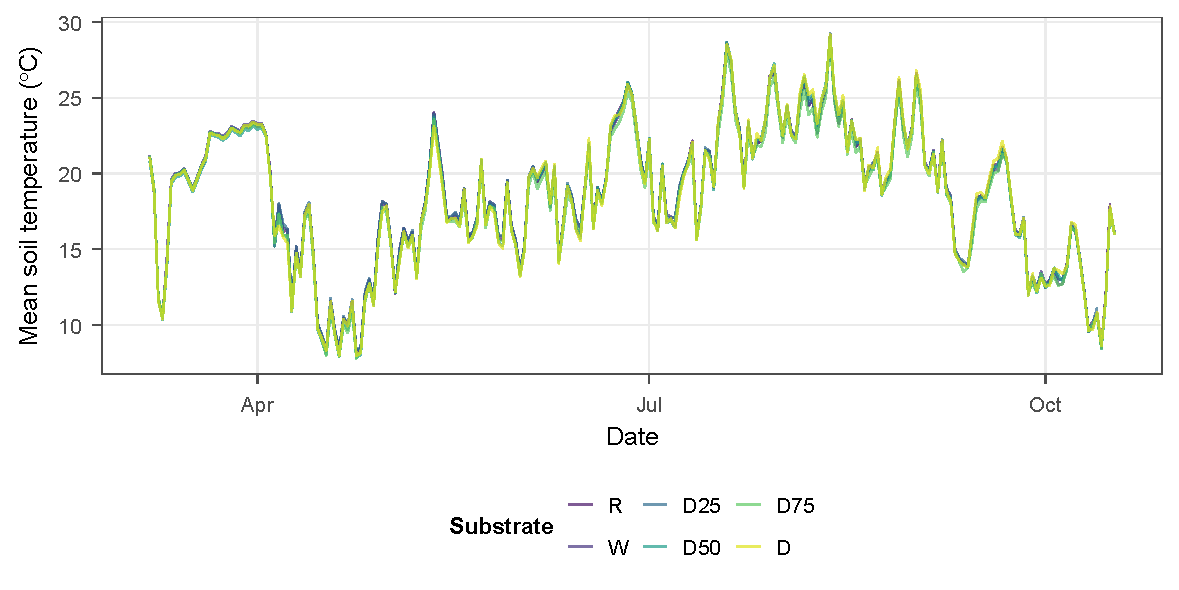
\includegraphics[width=\textwidth]{soil_temperature_timeseries.pdf}
        \caption{Soil temperature time series}
        \label{fig:app_soil_temp}
    \end{subfigure}
    \par\vspace{1em}
    \begin{subfigure}[b]{0.85\textwidth}
        \centering
        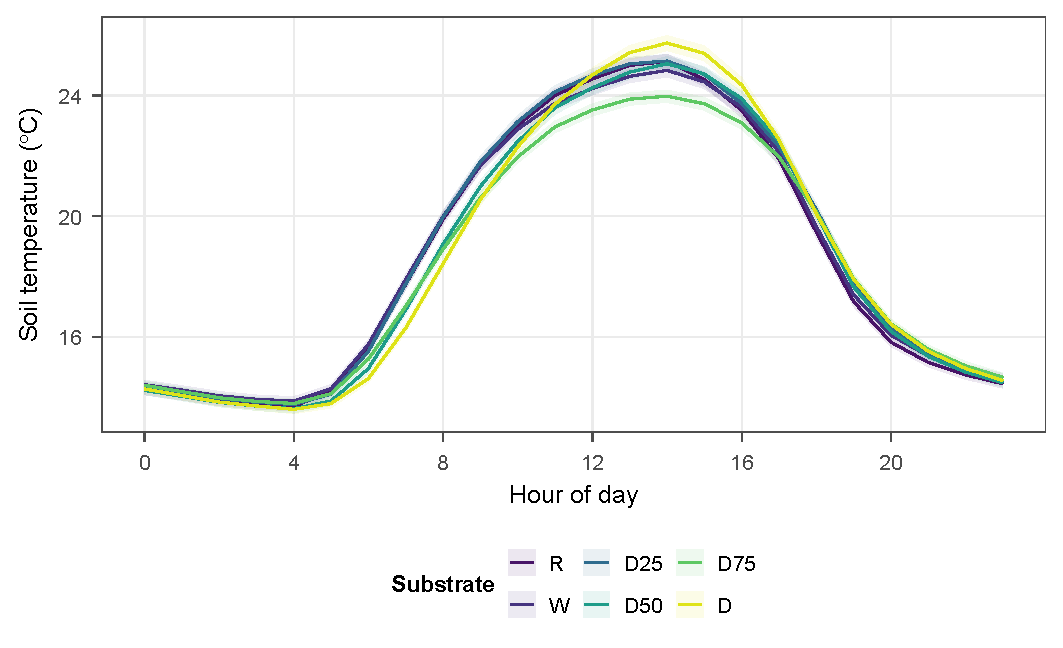
\includegraphics[width=\textwidth]{diurnal_temperature.pdf}
        \caption{Diurnal temperature range by substrate}
        \label{fig:app_temp_range}
    \end{subfigure}
    \caption{Temperature dynamics during the germination experiment: (a) daily mean soil temperature showing seasonal warming from April to August, with no significant substrate differences, and (b) diurnal temperature amplitude highlighting minor substrate-specific thermal buffering.}
    \label{fig:app_temperature_logs}
\end{figure}

\begin{figure}[htbp]
    \centering
    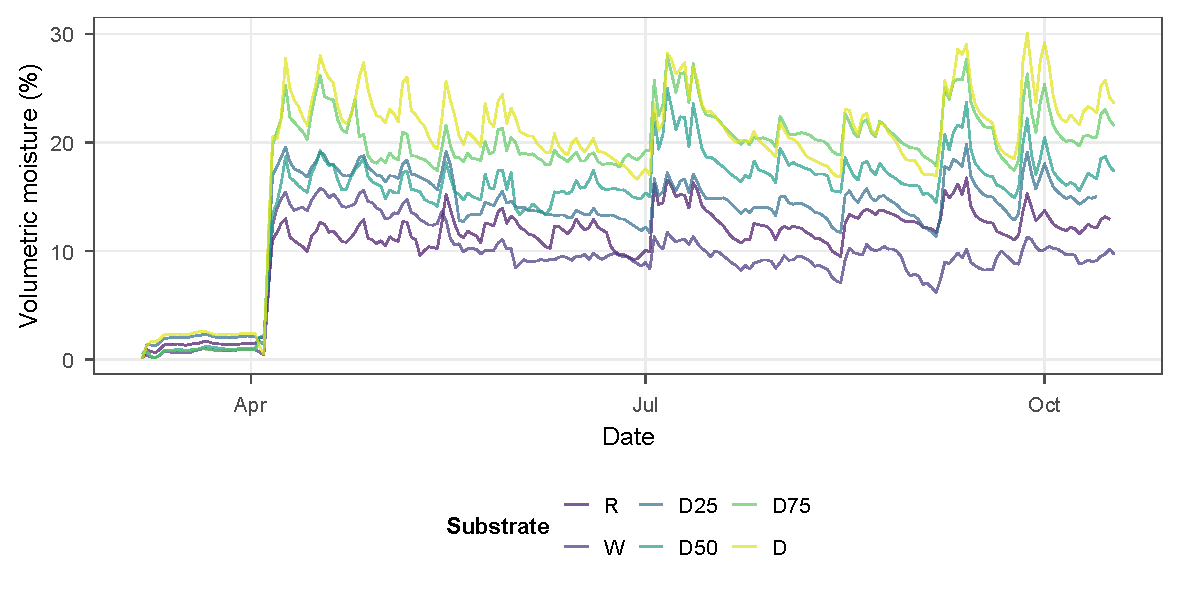
\includegraphics[width=0.65\textwidth]{soil_moisture_timeseries.pdf}
    \caption{Volumetric soil moisture time series by substrate, demonstrating the persistent moisture gradient attributable to the SOM ``sponge effect''. The dark substrate (D) maintained consistently higher moisture ($\overline{m} = 19.2\%$) than the reference beach sand (R, $\overline{m} = 10.8\%$).}
    \label{fig:app_moisture_timeseries}
\end{figure}


% --- Supplementary Tables ---
\clearpage
\section{Supplementary Tables}
\label{sec:appendix_tables}

% --- Substrate characterisation tables ---
\begin{table}[htbp]
\centering
\caption{Wilcoxon rank-sum test results comparing sediment properties between alternative (dredged) and control (beach) substrates, and between inside and outside sampling positions within the alternative substrate.}
\label{tab:substrate_stats}
\small
\begin{tabular}{l l r r}
\toprule
Comparison & Property & $W$ & $p$-value \\
\midrule
Alternative vs Control & TOC (\%) & 55 & 1.64e-08 \\
Alternative vs Control & TN (\%) & 176 & 1.34e-05 \\
Alternative vs Control & $D_{50}$ ($\mu$m) & 840 & 0.00634 \\
\midrule
Inside vs Outside & TOC (\%) & 517 & 0.75 \\
Inside vs Outside & TN (\%) & 562 & 0.808 \\
Inside vs Outside & $D_{50}$ ($\mu$m) & 560 & 0.828 \\
\bottomrule
\end{tabular}
\end{table}


\begin{table}[htbp]
\centering
\caption{Physical and chemical properties of the 10 experimental substrates used in the common garden experiment.}
\label{tab:substrate_summary}
\small
\begin{tabular}{l r r r l}
\toprule
Substrate & TOC (\%) & TN (\%) & $D_{50}$ ($\mu$m) & Description \\
\midrule
Ref          & 0.06 & 0.036 & 267 & Control (Natural Sand) \\
White        & 0.25 & 0.073 & 188 & Pure White Dredged Material \\
12.5% D      & 0.49 & 0.087 & 187 & Mixture \\
25% D        & 0.73 & 0.101 & 187 & Mixture \\
37.5% D      & 0.97 & 0.116 & 186 & Mixture \\
50% D        & 1.21 & 0.130 & 185 & Highest Growth Potential \\
62.5% D      & 1.45 & 0.144 & 185 & Mixture \\
75% D        & 1.68 & 0.159 & 184 & Mixture \\
87.5% D      & 1.92 & 0.173 & 184 & Mixture \\
Dark         & 2.16 & 0.187 & 183 & Pure Dark Dredged Material \\
\bottomrule
\end{tabular}
\end{table}


% --- Aboveground growth tables ---
\begin{table}[htbp]
\centering
\caption{Estimated marginal means (EMMs) for aboveground performance metrics. Height was modelled with a Gaussian LMM (quadratic time); leaf count with a Poisson GLMM (\texttt{glmmTMB}, quadratic time); both with plant identity as random intercept. Groups sharing the same letter are not significantly different (FDR-adjusted pairwise contrasts, $p < 0.05$).}
\label{tab:aboveground_lmm}
\small
\begin{tabular}{l rr cc}
\toprule
Substrate & Height EMM (cm) & Leaf count EMM & Height group & Leaf group \\
\midrule
R        & 43.9 & 8.8 & a & ab \\
D12.5    & 49.8 & 6.7 & ab & a \\
W        & 51.1 & 7.5 & ab & ab \\
D62.5    & 51.4 & 8.8 & ab & ab \\
D        & 53.3 & 12.2 & ab & b \\
D75      & 55.4 & 10.5 & b & ab \\
D87.5    & 56.6 & 10.1 & b & ab \\
D25      & 56.8 & 8.4 & b & ab \\
D37.5    & 57.7 & 8.1 & b & ab \\
D50      & 59.4 & 8.9 & b & ab \\
\bottomrule
\end{tabular}
\end{table}


% --- Belowground biomass tables ---
\begin{table}[htbp]
\centering
\caption{Statistical tests for belowground biomass metrics across the SOM gradient. Gamma GLM (log link) was fitted where data were strictly positive; Kruskal-Wallis is reported in parallel as a non-parametric reference. Benjamini-Hochberg correction applied to pairwise comparisons.}
\label{tab:belowground_stats}
\small
\begin{tabular}{l l r r r}
\toprule
Response & Method & Statistic & df & $p$-value \\
\midrule
Total root biomass & KW & $\chi^2$ = 6.87 & 9 & 0.65 \\
                   & Gamma & F = 0.68 & 9 & 0.724 \\
Root:shoot ratio & KW & $\chi^2$ = 9.67 & 9 & 0.377 \\
                 & Gamma & F = 1.41 & 9 & 0.219 \\
Shoot biomass & KW & $\chi^2$ = 5.76 & 9 & 0.764 \\
              & Gamma & F = 0.43 & 9 & 0.913 \\
\bottomrule
\end{tabular}
\end{table}


\begin{table}[htbp]
\centering
\caption{Belowground biomass and root:shoot ratio per substrate (mean $\pm$ SD). Statistical tests: Gamma GLM (log link) where feasible; Kruskal-Wallis rank-sum otherwise. See \cref{tab:belowground_stats} for test details.}
\label{tab:belowground_summary}
\small
\begin{tabular}{l r rr rr rr}
\toprule
Substrate & $n$ & Root (g) & & Shoot (g) & & R:S ratio & \\
          &     & Mean & SD & Mean & SD & Mean & SD \\
\midrule
R        & 2 & 4.49 & 0.01 & 4.12 & 0.35 & 1.09 & 0.09 \\
W        & 3 & 6.76 & 3.64 & 4.74 & 1.64 & 1.37 & 0.30 \\
D12.5    & 6 & 7.51 & 5.63 & 4.79 & 2.32 & 1.51 & 0.62 \\
D25      & 5 & 5.96 & 0.92 & 5.42 & 1.02 & 1.12 & 0.22 \\
D37.5    & 6 & 7.12 & 3.10 & 5.89 & 1.56 & 1.23 & 0.52 \\
D50      & 6 & 6.05 & 2.46 & 5.79 & 2.32 & 1.12 & 0.39 \\
D62.5    & 6 & 5.98 & 0.80 & 4.96 & 1.45 & 1.29 & 0.37 \\
D75      & 6 & 5.83 & 3.03 & 4.83 & 2.59 & 1.42 & 0.60 \\
D87.5    & 5 & 4.43 & 2.44 & 5.41 & 2.54 & 0.78 & 0.49 \\
D        & 2 & 4.37 & 0.59 & 5.87 & 0.55 & 0.75 & 0.17 \\
\bottomrule
\end{tabular}
\end{table}


% --- Germination tables ---
\begin{table}[htbp]
\centering
\caption{Germination and seedling establishment across substrates. Germination at $t_1$ (10 seeds per pot, $n=16$) modelled with a binomial GLM (quasibinomial due to overdispersion); seedling count over time modelled with a Negative Binomial GLMM (\texttt{glmmTMB}, quadratic time, random intercept per pot). Groups sharing the same letter are not significantly different (FDR-adjusted pairwise contrasts, $p < 0.05$).}
\label{tab:germination_stats}
\small
\begin{tabular}{l r rr rr cc}
\toprule
Substrate & $n$ & Germ. \% & SD & EMM count & SE & Germ. group & Count group \\
\midrule
R      & 16 & 6.2 & 13.6 & 0.4 & 0.1 & a & a \\
W      & 16 & 53.1 & 21.8 & 3.4 & 0.7 & c & bc \\
D25    & 16 & 46.9 & 18.2 & 4.0 & 0.7 & c & bc \\
D50    & 16 & 49.4 & 22.6 & 3.7 & 0.7 & c & bc \\
D75    & 16 & 54.4 & 25.3 & 4.7 & 0.8 & c & c \\
D      & 16 & 23.1 & 22.4 & 2.2 & 0.5 & b & b \\
\bottomrule
\end{tabular}
\end{table}


% --- Microclimate tables ---
\begin{table}[htbp]
\centering
\caption{Microclimate conditions in germination experiment substrates, measured by TMS-4 loggers. Values are daily means $\pm$ SD.}
\label{tab:microclimate}
\small
\begin{tabular}{l r l l l}
\toprule
Substrate & Days & Soil temp. ($^{\circ}$C) & Air temp. ($^{\circ}$C) & Vol. moisture (\%) \\
\midrule
R      & 224 & 18.6 +/- 4.5 & 17.2 +/- 4.0 & 10.8 +/- 3.9 \\
W      & 225 & 18.7 +/- 4.5 & 17.1 +/- 4.1 & 9.1 +/- 3.8 \\
D25    & 221 & 18.8 +/- 4.4 & 17.3 +/- 4.0 & 13.3 +/- 4.8 \\
D50    & 225 & 18.5 +/- 4.6 & 17.2 +/- 4.1 & 14.9 +/- 5.7 \\
D75    & 225 & 18.4 +/- 4.4 & 17.3 +/- 4.0 & 18.1 +/- 7.0 \\
D      & 225 & 18.6 +/- 4.6 & 17.2 +/- 4.0 & 19.2 +/- 7.2 \\
\bottomrule
\end{tabular}
\end{table}


% --- SOM response model tables ---
\begin{table}[htbp]
\centering
\caption{Non-linear regression coefficients for the Gaussian growth response models (Levenberg--Marquardt algorithm). The response function is $y = b_0 + a \cdot \exp\left(-\frac{(\mathrm{SOM} - \mu)^2}{2\sigma^2}\right)$, where $b_0$ is the baseline multiplier, $a$ is the amplitude, $\mu$ is the optimal SOM (\% TOC), and $\sigma$ is the standard deviation of the response. Response variables are normalised to the reference beach sand (R). $\dagger$~Including outlier plant 6b\_5 (97 leaves). $\ddagger$~Outlier removed; amplitude non-significant.}
\label{tab:growth_coefficients}
\small
\begin{tabular}{ll rrrr rr r}
\toprule
Response & Parameter & Estimate & SE & $t$ & $p$ & $R^2$ & $R^2_{adj}$ & $n$ \\
\midrule
Height & $b0$ & 0.5000 & 4.3047 & 0.12 & 0.911 & 0.659 & 0.387 & 120 \\
 & $amp$ & 0.8070 & 4.2818 & 0.19 & 0.857 &  &  &  \\
 & $mu$ & 1.3227 & 0.1441 & 9.18 & $<$0.001 &  &  &  \\
 & $sigma$ & 1.5181 & 4.7023 & 0.32 & 0.758 &  &  &  \\
\midrule
Density$^\dagger$ & $b0$ & 1.0331 & 0.0348 & 29.65 & $<$0.001 & 0.639 & 0.349 & 120 \\
 & $amp$ & 1.4019 & 1.6486 & 0.85 & 0.428 &  &  &  \\
 & $mu$ & 0.6480 & 0.0689 & 9.41 & $<$0.001 &  &  &  \\
 & $sigma$ & 0.1000 & 0.0893 & 1.12 & 0.305 &  &  &  \\
\midrule
Density (clean)$^\ddagger$ & $b0$ & 1.0447 & 0.0357 & 29.24 & $<$0.001 & 0.532 & 0.157 & 119 \\
 & $amp$ & 0.2330 & 0.1374 & 1.70 & 0.141 &  &  &  \\
 & $mu$ & 0.5014 & 0.2245 & 2.23 & 0.067 &  &  &  \\
 & $sigma$ & 0.1000 & 0.1082 & 0.92 & 0.391 &  &  &  \\
\midrule
Root & $b0$ & 0.8858 & 0.8063 & 1.10 & 0.314 & 0.544 & 0.18 & 228 \\
 & $amp$ & 0.6523 & 0.7566 & 0.86 & 0.422 &  &  &  \\
 & $mu$ & 1.2423 & 0.1555 & 7.99 & $<$0.001 &  &  &  \\
 & $sigma$ & 0.6773 & 0.7599 & 0.89 & 0.407 &  &  &  \\
\bottomrule
\end{tabular}
\end{table}


\begin{table}[htbp]
\centering
\caption{Binomial GLMM coefficients for the survival--SOM relationship. The model is $\mathrm{logit}(P_{\mathrm{survival}}) = \beta_0 + \beta_1 \cdot \mathrm{SOM} + u_j$, where $u_j \sim \mathcal{N}(0, \sigma^2_u)$ is a random intercept for spatial block $j$ (column position in common garden). McFadden pseudo-$R^2$:  0 .}
\label{tab:mortality_coefficients}
\begin{tabular}{lrrrr}
\toprule
Component & Estimate & SE & $z$ & $p$ \\
\midrule
\multicolumn{5}{l}{\textit{Fixed effects}} \\
$\beta_0$ (Intercept) & 1.3236 & 0.4252 & 3.11 & 0.0019 \\
$\beta_1$ (SOM) & 0.0105 & 0.3314 & 0.03 & 0.9748 \\
\midrule
\multicolumn{5}{l}{\textit{Random effects}} \\
$\sigma_u$ (column) & 0.0000 & & & \\
\midrule
\multicolumn{5}{l}{\textit{Derived Living Dunes parameters}} \\
Steepness ($-\beta_1$) & -0.0105 & & & \\
Threshold ($-\beta_0/\beta_1$) & -126.21 & & & \\
\bottomrule
\end{tabular}
\end{table}


\begin{table}[htbp]
\centering
\caption{Model fit statistics for the SOM response curve derivations. Growth models use non-linear least squares with the Levenberg--Marquardt algorithm (\texttt{nlsLM}). The mortality model uses a binomial generalised linear mixed model (GLMM) with a random intercept for spatial block.}
\label{tab:model_fit_statistics}
\begin{tabular}{l r r r r r}
\toprule
Model & Log-Lik & AIC & $\sigma_\varepsilon$ & $R^2$ & $n$ \\
\midrule
Height NLS & 14.6 & -19.3 & 0.4022 & 0.659 & 120 \\
Density NLS & 10.5 & -10.9 & 0.5916 & 0.639 & 120 \\
Root NLS & 4.0 & 2.0 & 0.5492 & 0.544 & 228 \\
Mortality GLMM & -61.4 & 128.8 & --- & 0.000$^\dagger$ & 120 \\
\bottomrule
\multicolumn{6}{l}{\footnotesize $\dagger$ McFadden pseudo-$R^2$ for the binomial GLMM.} \\
\end{tabular}
\end{table}



\end{document}
